\documentclass[11pt,a4paper]{article}
\usepackage[margin=2.4cm]{geometry}
\usepackage{amsmath,amssymb,mathtools}
\usepackage{graphicx,booktabs,xcolor,tabularx,array}
\usepackage{tikz}
\usetikzlibrary{arrows.meta,positioning}
\usepackage{algorithm}
\usepackage[noend]{algpseudocode}
\usepackage[hidelinks]{hyperref}

\definecolor{rl}{HTML}{2A78D6}
\definecolor{ink2}{HTML}{52514E}
\algrenewcommand\algorithmiccomment[1]{\hfill{\small$\triangleright$ #1}}
\setlength{\emergencystretch}{1.5em}
\renewcommand{\topfraction}{0.9}\renewcommand{\bottomfraction}{0.8}\renewcommand{\textfraction}{0.07}
\renewcommand{\floatpagefraction}{0.7}\setcounter{topnumber}{2}\setcounter{totalnumber}{4}

% Statements as in RL-TR-2026-03 (amsthm "plain" and "definition" styles): the name in bold, the note in
% parentheses, a bold period, then the body, italic for results and upright for definitions.
\NewDocumentEnvironment{result}{m o}
  {\par\medskip\noindent\textbf{#1}\IfValueT{#2}{ (#2)}\textbf{.}\enspace\itshape\ignorespaces}{\par\medskip}
\NewDocumentEnvironment{defn}{m o}
  {\par\medskip\noindent\textbf{#1}\IfValueT{#2}{ (#2)}\textbf{.}\enspace\ignorespaces}{\par\medskip}
\newenvironment{proof}{\par\noindent\textit{Proof.}\enspace\ignorespaces}
  {\leavevmode\unskip\penalty9999\hbox{}\nobreak\hfill\quad\hbox{$\square$}\par\medskip}

\newcommand{\Vs}{V^\star}
\newcommand{\E}{\mathcal E}
\newcommand{\code}[1]{\texttt{\detokenize{#1}}}
\newcommand{\trace}[4]{\par\smallskip\noindent{\small\raggedright\emph{Code} #1\enspace\textperiodcentered\enspace
  \emph{Lean} #2\enspace\textperiodcentered\enspace\emph{Check} #3\enspace\textperiodcentered\enspace\emph{Bench} #4\par}\medskip}
\newcolumntype{L}{>{\raggedright\arraybackslash}X}
\DeclarePairedDelimiter\abs{\lvert}{\rvert}
\DeclarePairedDelimiter\norm{\lVert}{\rVert}

\title{\textbf{GRACE-3D 2.0.0}: Goal-Relevant Adaptive Compressed Exchange in three dimensions\\[2pt]
\large Navigating unknown voxel worlds and telling teammates only what changes their decision,\\
with 228 bytes of state, one millisecond per slot and no global coordinates}
\author{Ropera Labs\\\small Technical report RL-TR-2026-04 \textperiodcentered{} swarm-dil v2.0.0}
\date{November 2026}

\begin{document}
\maketitle

\begin{abstract}
GRACE (RL-TR-2026-03) derived what memory-limited agents crossing unknown terrain should tell each other, on a
two-dimensional grid. GRACE-3D 2.0.0 (``v2'' below) moves it to a 26-connected voxel lattice under the budget of a 168\,MHz
microcontroller: 228 bytes of persistent state, 168\,000 cycles per one-second slot, and a packet header that
carries no global coordinate. We give the lattice metric in closed form; a tile code within a constant factor of
the information bound; an ingestion cost whose reading term every correct agent must pay; exact replanning by a
time-sliced A* whose every intermediate value is a sound lower bound on the true cost-to-go; a 15-bit wrapped pose
that decodes exactly after up to 15 slots of silence; and arrival with probability one for any memory bound and any
received content, which is the best a single agent can have, since no finite-state deterministic agent finds the goal
in every world. One post-empirical pass adds a futility trigger, proved sound and adopted after a paired test on 40
terrains whose decision rule was fixed before the runs. Every result is proved in full here; the structural core is
mechanised in Lean~4 and the rest is checked symbolically, exhaustively or by Monte Carlo. In simulation, ten agents
keep the regret of GRACE ported to 3-D (given 120 bytes of map) and never exceed 228\,B of state or 0.74\,ms of
modelled compute per slot.
\end{abstract}

\begin{figure}[htbp]\centering
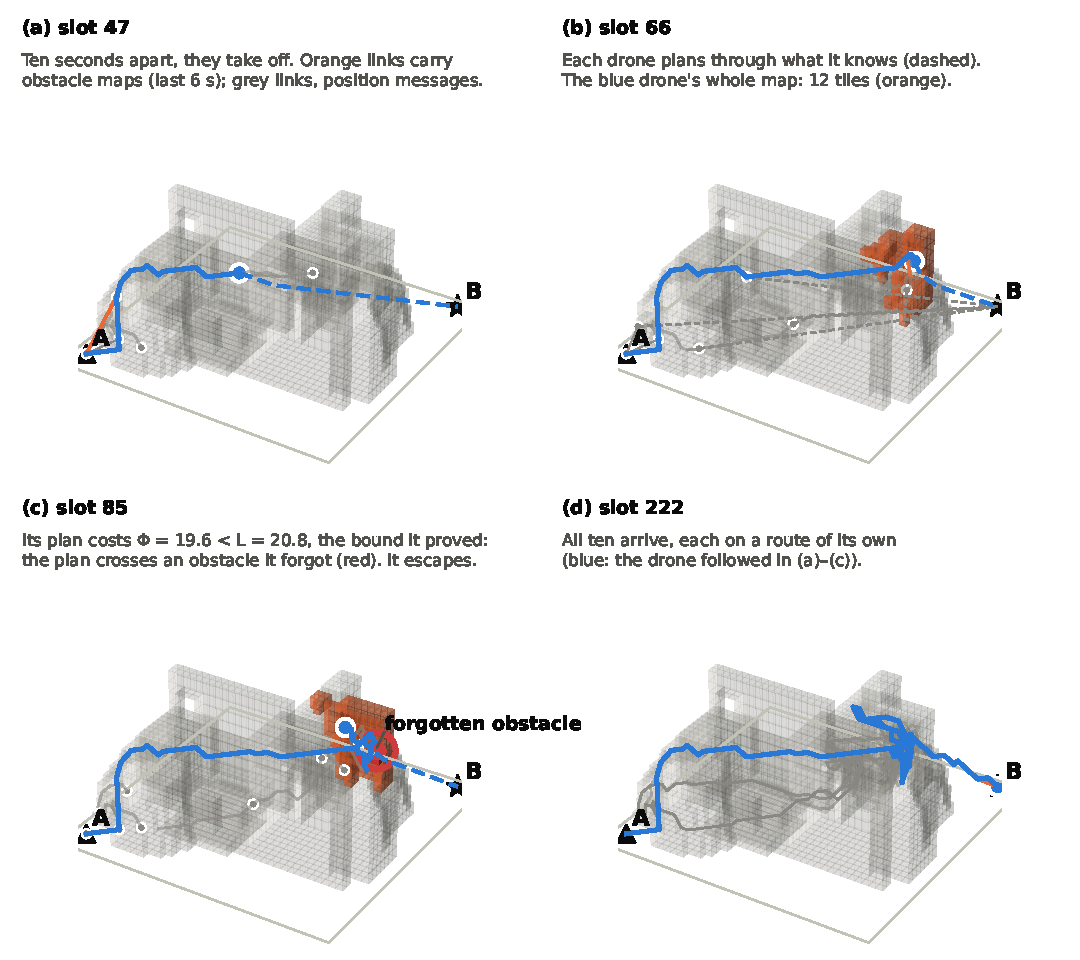
\includegraphics[width=\linewidth]{fig/swarm_strip.pdf}
\caption{GRACE-3D 2.0.0 at work, one recorded mission (seed 2, regret 0.88; the mean over the 20 bench terrains is
0.99). The drone followed is blue, its teammates grey, the ground-truth obstacles a faint grey. (a) The team takes off
ten seconds apart; orange links are radio packets carrying obstacle maps, grey links short position messages. (b) Each
drone plans its own route through what it knows (dashed); the blue drone's entire map is the 12 tiles shown in orange.
(c) Its new plan costs less than the lower bound it has proved, so it must cross a real obstacle: one the drone held
a second earlier and evicted (red, Theorems F45.1--F45.2). It escapes at once. (d) All ten arrive. The animated
version is \code{results/v2/grace3d_swarm.gif}; the explainer page replays it in 3-D.}
\label{fig:strip}
\end{figure}

\section{Problem and contributions}\label{sec:claim}

\paragraph{Operational setting.} GRACE~\cite{v1} derived what memory-limited agents crossing unknown terrain should tell
each other, on a two-dimensional grid. GRACE-3D 2.0.0 asks whether that principle survives three dimensions on the
budget of a small flight controller. A team of $N=10$ agents crosses an unknown voxel world from $A$ to $B$. Each agent
has 256 bytes of persistent state, one millisecond of a 168\,MHz Cortex-M4 per one-second slot, two $8\times8$
time-of-flight zone sensors, and a radio whose packet header may carry no global coordinate. Cycle figures come from a
declared operation-count model of that processor (Section~\ref{sec:budget}), not from hardware.

\paragraph{Design principle.} As in GRACE, an agent plans as if the unknown were free, so only obstacles can change its
plan, and only obstacles are stored and sent. What is new is that a 256-byte agent must forget, and forgetting must
neither trap an agent nor mislead it: every search proves a lower bound on the true distance; a tile is evicted only
if it cannot change the current plan; a plan cheaper than the proved bound exposes a harmful eviction; and a random
escape keeps arrival certain, with probability one, whatever is forgotten or received.

\paragraph{Contributions.}
\begin{enumerate}
\item The exact distance of the 26-connected lattice in closed form, and canonical segments that realise it within one
voxel of the straight line (Lemma H.1--H.5, Theorem T2.5a).
\item A $4\times4\times4$ tile code within a constant factor of the information bound, whose merge is a bitwise OR that
commutes with translation, so maps need no global frame (T2.1, T2.3); and a 15-bit wrapped pose that decodes exactly
after up to 15 slots of silence (T2.4).
\item An ingestion cost whose reading term every correct agent must pay (T2.2).
\item Exact replanning in a fixed arena by an A* sliced over slots, whose every intermediate value is a sound lower
bound, and a forgetting rule that cannot change the current plan (T2.6, T2.7).
\item Arrival with probability one for any memory bound and any received content, deterministic arrival along a
verified route, and the impossibility of deterministic completeness with finite state (T2.8--T2.10); and a futility
trigger, proved sound and adopted by a pre-registered paired test (F45.1--F45.6, Section~\ref{sec:f45}).
\item The protocol itself, in 228 bytes and at most 124\,954 modelled cycles per slot (Section~\ref{sec:protocol},
Algorithms~\ref{alg:slot}--\ref{alg:send}), and a paired study on 20 terrains against GRACE ported to 3-D, CAIRN
v0.4, flooding and silence (Section~\ref{sec:measure}).
\end{enumerate}
Table~\ref{tab:targets} maps the targets set for v2 to these results.

\paragraph{Related work.} No finite automaton searches every finite plane labyrinth (Budach~\cite{budach}; see
also~\cite{hoffmann}); every $K$-state automaton has a planar trap with at most $K+1$ nodes~\cite{fipp}; two
cooperating automata are reported to suffice in the plane~\cite{blumkozen}; deterministic log space decides undirected
connectivity~\cite{reingold}; and a random walk covers every connected graph~\cite{aleliunas}. In three dimensions the
range-sensor algorithm 3DBug is globally convergent, but it ends up holding the whole obstacle surface that blocks
it~\cite{kamon}, so its memory grows with the obstacle. Incremental replanning (Ramalingam and Reps~\cite{rr96},
D*~Lite~\cite{dstarlite}) keeps a distance per vertex, $\Theta(\abs\Omega)$ state, while A*~\cite{hart} run from the
current state needs only scratch memory. Merges that tolerate duplication and reordering are joins of a semilattice,
as in conflict-free replicated data types~\cite{shapiro}. Multizone time-of-flight sensors already drive obstacle
avoidance on a Crazyflie~2.1 with a 168\,MHz STM32F405, in 210\,\textmu s per frame~\cite{muller}; that sensor and
processor set the hardware model here. To our knowledge, no prior work bounds the memory of an optimistic planner that
forgets, uses its searches' lower bounds as the certificates it communicates, or sends a few-byte header with no
absolute coordinate.

\paragraph{How to read this report.} Section~\ref{sec:idea} explains the algorithm in plain words,
Section~\ref{sec:model} fixes the model and Section~\ref{sec:protocol} the exact rules, with pseudocode.
Section~\ref{sec:results} proves every result in full, and each result ends with its trace: the code that implements
it, the Lean theorems that mechanise it (\code{formal/v2_theorems.lean}, Lean 4.36 and Mathlib v4.36.0, no
\code{sorry}, axioms \code{propext}, \code{Classical.choice} and \code{Quot.sound} only), the check in
\code{tests/math_verify_v2.py} or \code{tests/test_sim3d.py}, and the benchmark quantity (Section~\ref{sec:measure}).

\begin{table}[htbp]\centering\small
\begin{tabularx}{\linewidth}{>{\raggedright\arraybackslash}p{3.6cm}L>{\raggedright\arraybackslash}p{2.2cm}}
\toprule
v2 target & Result & Where \\
\midrule
3-D space, information efficiency $\eta=O(1)$ against 2-D & exact lattice metric $h_3$; $4\times4\times4$ tiles at
$0.625$\,B per surface voxel in expectation, 0.641\,B measured; $\eta_{3D}/\eta_{2D}=$\,1.05 & H.1--H.5, T2.1, C1 \\
perception $O(\abs{\Delta O_{\rm visible}})$ & $P$ zone reads, a lower bound for every correct agent, plus
$\abs{\Delta O}$ bit inserts; 1\,456 cycles at p99 & T2.2, C2 \\
incremental replanning within 256\,B and 1\,ms & exact A* on the believed lattice, sliced over slots on a frozen map,
every value a sound lower bound; 228\,B of persistent state; at most 124\,152 of 168\,000 cycles per slot, no
overrun in 43\,406 agent-slots & T2.6, T2.7, T2.11, C3 \\
header without GNSS, 0\,B of global coordinates & 5-byte header, 15-bit wrapped pose, exact after up to 15 slots of
silence; merging commutes with translation & T2.3, T2.4, C4 \\
completeness & probability one for any memory bound and any received content; deterministic along a verified route;
deterministic completeness with finite state is impossible & T2.8--T2.10 \\
\bottomrule
\end{tabularx}
\caption{The targets set for v2, the result that meets each, and where it is proved (Section~\ref{sec:results}) or
measured (C1--C4, Section~\ref{sec:measure}).}
\label{tab:targets}
\end{table}

\section{How GRACE-3D 2.0.0 works, in plain words}\label{sec:idea}

Ten drones leave $A$ one after another, ten seconds apart, and must reach $B$ through a world none of them has seen
(Figure~\ref{fig:strip}). Each has a short-range depth sensor (5 voxels, 25\,m), a weak shared radio, 256 bytes of
memory and one millisecond of a small processor per second. Eight ideas make that enough; Section~\ref{sec:protocol}
gives the exact rules and their pseudocode, Section~\ref{sec:results} the proofs.

\paragraph{1. Plan as if the unknown were free.} A drone plans the shortest route to $B$ assuming that every voxel it
does not know to be blocked is free. Learning that a voxel is free could then never change its plan, so free space is
never stored or sent: memory and radio carry obstacles only. A plan is a list of at most 8 waypoints. Between two
waypoints the drone flies a fixed pattern of unit steps, the canonical segment $\sigma$, whose length is exactly the
lattice distance $h_3$ (Section~\ref{sec:segment}).

\paragraph{2. Every search proves a lower bound.} The obstacles a drone holds are real: it sensed them, or an honest
teammate did. A map with fewer obstacles than the world can only make routes look shorter, so the shortest route
through the drone's map, of length $d_K$, is never longer than the true one, $\Vs$. Each planning search therefore
proves a number $L$ with $L\le\Vs$: the drone \emph{knows} it cannot reach $B$ in less than $L$. After a step of
length $c$ the number $L-c$ is still a valid bound, so the knowledge is kept, not recomputed (T2.0, T2.6).

\paragraph{3. Twelve tiles of map, and a rule for what to forget.} Obstacles are stored in $4\times4\times4$-voxel tiles
of 10 bytes each, and a drone holds at most 12 (Figure~\ref{fig:strip}b). When a thirteenth arrives, it evicts the
tile that matters least: the one farthest outside the region of voxels that a route as cheap as its current plan
could pass through. A tile outside that region cannot change the current plan (T2.7). Tiles touched in the current
second are evicted only if every tile was, so a drone does not forget what it is about to hit.

\paragraph{4. An exact search that fits in one millisecond.} A* finds the shortest route through the drone's map, but
may need more than a millisecond. So it expands as many nodes as fit in 70\,\% of each second's budget, while the drone
hovers and its map is frozen, and resumes in the next second. Even unfinished, the search's lowest current estimate is
already a valid bound $L$ (T2.6). The path found is compressed into a few long canonical segments.

\paragraph{5. A plan that is too cheap to be true.} Forgetting has a price: a drone may plan straight through an
obstacle it held and evicted. GRACE-3D 2.0.0 detects this exactly. The plan's cost $\Phi$ is the length of a route;
the bound $L$ says that no route to $B$ is shorter than $L$. If $\Phi<L$, the plan cannot be a real route, so it must
cross a real obstacle (Theorem F45.1), and with honest maps this can only happen after an eviction (F45.2). The drone
drops the plan at once and escapes (Figure~\ref{fig:futility}).

\paragraph{6. Never stuck for ever.} With so little memory a drone can circle. When a decision makes no progress (the
plan's cost did not drop by at least one voxel) and nothing new was learned, the drone starts, with probability 5\,\%,
an \emph{escape}: a random walk that keeps its direction most of the time, avoids known obstacles half of the time and
lasts four seconds on average. This guarantees arrival with probability one, whatever the memory size and whatever
teammates say (T2.9).

\paragraph{7. Tell teammates only what changes their route.} A drone offers a tile only if that tile refuted one of its
own plans, and sends it only if the detour it would save teammates still flying is worth more than its 10 bytes: the
value of a tile to a teammate is twice the distance that teammate would fly before seeing the obstacle itself,
discounted by how far the tile lies off the teammate's way to $B$ (GRACE, Proposition~1). Every 10 seconds a flying
drone also announces its cell and next two waypoints (PLAN), and an arrived drone whose flown route fits in 12 waypoints
shares that route (VERIFIED).

\paragraph{8. No global coordinates on the radio.} Positions are counted from $A$ by dead reckoning. A packet carries its
sender's position modulo 32 voxels on each axis (15 bits); the receiver recovers the exact position from its previous
estimate, as long as it heard the sender within the last 15 seconds (T2.4). Maps merge by bitwise OR, so the order,
repetition and relaying of packets never matter (T2.3).

\begin{table}[htbp]\centering\small
\begin{tabularx}{\linewidth}{>{\raggedright\arraybackslash}p{3.2cm}L}
\toprule
Symbol & Meaning \\
\midrule
$\Omega$, $O$ & the voxel world, and its blocked voxels (unknown to the agents) \\
$A$, $B$, $p_i$ & start, goal, and the position of agent $i$ \\
$S$ & the 26 unit steps: each coordinate changes by $-1$, $0$ or $+1$, not all zero \\
$h_3(d)$ & the length of a shortest walk across the displacement $d$ in empty space \\
$K$, $K_i$ & a set of voxels believed blocked; the voxels agent $i$ holds. As a number, $K$ is the tile budget
(12; 6 in the stress test) \\
$G(K)$, $d_K(x)$ & the lattice without the voxels of $K$; the length of a shortest walk from $x$ to $B$ in it \\
$\Vs(x)=d_O(x)$ & the true remaining distance from $x$ to $B$ \\
$L_i$ & agent $i$'s proven lower bound on $\Vs(p_i)$ \\
$\Phi$ & the cost of agent $i$'s current plan (the length of the whole route it planned) \\
$\E(x,B,U)$ & the voxels through which some walk from $x$ to $B$ of cost at most $U$ can pass \\
$\sigma(p,q)$ & the canonical segment: the fixed list of unit steps from $p$ to $q$ \\
$r$, $\kappa$ & sensor range (5 voxels); price of one byte, in voxels of detour it must save \\
$p_{\rm esc}$, $\rho$, $\mu$ & escape probability (0.05), re-draw probability per step (0.25), mean escape length (4) \\
regret & (distance flown + true distance left) / $\Vs(A)$ $-$ 1, averaged over the team \\
\bottomrule
\end{tabularx}
\caption{Notation.}\label{tab:notation}
\end{table}

\section{Model}\label{sec:model}

\begin{defn}{(W) World}
$\Omega=\{0..n_x-1\}\times\{0..n_y-1\}\times\{0..n_z-1\}\subset\mathbb Z^3$ (default $40\times40\times10$ voxels of
5\,m); a static blocked set $O\subset\Omega$; start $A$ and goal $B$ free. Unit steps $S=\{-1,0,1\}^3\setminus\{0\}$. A
move from $x$ by $s\in S$ succeeds iff $x+s\in\Omega\setminus O$, and the agent observes whether it did.
\end{defn}

\begin{defn}{(C) Costs}
$a_1=1$, $a_2=\sqrt2-1$, $a_3=\sqrt3-\sqrt2$, and $h_3(d)=a_1\delta_1+a_2\delta_2+a_3\delta_3$ with
$\delta_1\ge\delta_2\ge\delta_3$ the sorted $\abs{d_x},\abs{d_y},\abs{d_z}$. A step $s$ costs $c(s)=h_3(s)$, that is
$1,\sqrt2,\sqrt3$ for 1, 2, 3 non-zero coordinates. A walk $x_0,\dots,x_n$ has $x_k-x_{k-1}\in S$, costs
$\sum_kc(x_k-x_{k-1})$ and \emph{enters} $x_1,\dots,x_n$.
\end{defn}

\noindent\emph{Why these weights.} A step costs its Euclidean length. In empty space the cheapest way across a
displacement $d$ moves along all three axes at once for $\delta_3$ steps (cost $\sqrt3$ each), then along the two
largest for $\delta_2-\delta_3$ steps ($\sqrt2$ each), then along the largest alone for $\delta_1-\delta_2$ steps (1
each). The total, $\sqrt3\,\delta_3+\sqrt2\,(\delta_2-\delta_3)+(\delta_1-\delta_2)$, regrouped by $\delta$, is $h_3(d)$.
For example $d=(5,3,1)$ gives $\sqrt3+2\sqrt2+2=5+3(\sqrt2-1)+(\sqrt3-\sqrt2)\approx6.56$ voxels, against a Euclidean
length of $\sqrt{35}\approx5.92$: the lattice never stretches a straight line by more than 12.8\,\%.

\begin{defn}{(G) Graphs and bounds}
For $K\subseteq\Omega$, $G(K)$ has an arc $x\to x+s$ iff $x+s\in\Omega\setminus K$; $d_K(x)$ is the least cost of a walk
from $x$ to $B$ in $G(K)$ ($\infty$ if none), and $\Vs=d_O$. For $U\ge0$, the \emph{informed set} is
$\E(x,B,U)=\{y:h_3(y-x)+h_3(B-y)\le U\}$.
\end{defn}

\noindent\emph{In words.} $d_K(x)$ is the remaining distance an agent believes in when $K$ is everything it knows to be
blocked; $\Vs(x)$ is the true one. Because unknown voxels count as free, $d_K\le\Vs$ whenever $K$ holds only real
obstacles. The informed set is the lattice analogue of an ellipsoid with foci $x$ and $B$: a voxel belongs to it
exactly when going from $x$ to $B$ through that voxel could cost at most $U$.

\begin{defn}{(S) Sensing, messages and hardware}
Per slot, $P=128$ zones (two $8\times8$ time-of-flight arrays of $60^\circ$, one along the heading, one sideways and
rotating through four headings), each returning the first hit within $r=5$ voxels or ``none''; sensing is exact.
Received obstacle data are true (\emph{honest} teammates) wherever a result says so; T2.9 needs no such assumption.
Hardware class: Cortex-M4F at 168\,MHz; a slot lasts 1\,s and grants 168\,000 cycles; persistent state at most 256\,B;
one static scratch arena of 16\,KiB, never heap-allocated.
\end{defn}

\begin{defn}{Definition 1 of v1: isolation}
An agent's software uses only its mission order ($A$, $B$, team size, launch slot, limits), its own zone readings as
offsets from itself, whether its last move happened, and the raw bytes it receives. Positions are kept by dead
reckoning in the swarm frame $F_A$ (origin at $A$); no external frame appears anywhere.
\end{defn}

Kept from v1~\cite{v1}: optimistic planning (unknown means free), static obstacles, exact odometry, identical agents. Relaxed:
2-D grid to 3-D lattice; unbounded computation per slot to 1\,ms; unlimited map to 256\,B of state.

\section{The algorithm}\label{sec:protocol}

An \emph{acquisition} is a blocked voxel entering memory (sensed, revealed by a failed move, or received); it is
\emph{fresh} if its tile key is not in the eviction Bloom filter, that is, if the agent never held that tile before.
$\Phi$ is the cost of the remaining plan ($\infty$ without one). The eight steps below are the specification; the
pseudocode after them (Algorithms~\ref{alg:slot}--\ref{alg:send}) is how \code{src/sim3d/agent.py} implements them,
in the order it executes them. Figure~\ref{fig:flow} shows how the parts feed each other.

\begin{figure}[htbp]\centering
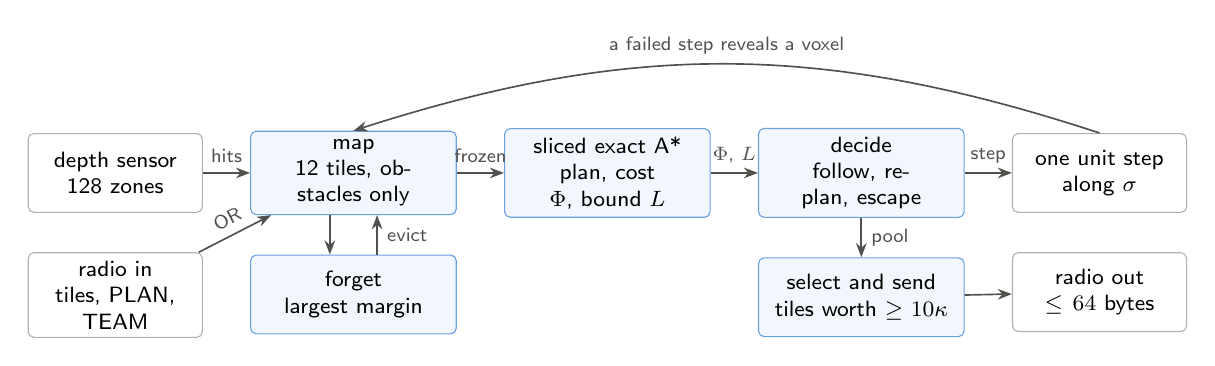
\begin{tikzpicture}[node distance=5mm and 6mm, every node/.style={font=\sffamily\footnotesize},
  part/.style={draw=rl!70,fill=rl!6,rounded corners=2pt,align=center,inner sep=3pt,minimum height=10mm,text width=24mm},
  io/.style={draw=ink2!45,fill=white,rounded corners=2pt,align=center,inner sep=3pt,minimum height=10mm,text width=20mm},
  arr/.style={-{Stealth[length=1.8mm]},draw=ink2,semithick}, lab/.style={font=\sffamily\scriptsize,text=ink2}]
  \node[io] (sense) {depth sensor\\128 zones};
  \node[part, right=of sense] (map) {map\\12 tiles, obstacles only};
  \node[part, right=of map] (plan) {sliced exact A*\\plan, cost $\Phi$, bound $L$};
  \node[part, right=of plan] (decide) {decide\\follow, re-plan, escape};
  \node[io, right=of decide] (move) {one unit step\\along $\sigma$};
  \node[io, below=of sense] (rxin) {radio in\\tiles, PLAN, TEAM};
  \node[part, below=of map] (forget) {forget\\largest margin};
  \node[part, below=of decide] (send) {select and send\\tiles worth $\ge10\kappa$};
  \node[io, below=of move] (rxout) {radio out\\$\le64$ bytes};
  \draw[arr] (sense) -- node[lab,above]{hits} (map);
  \draw[arr] (rxin) -- node[lab,above,sloped]{OR} (map);
  \draw[arr] ([xshift=-3mm]map.south) -- ([xshift=-3mm]forget.north);
  \draw[arr] ([xshift=3mm]forget.north) -- node[lab,right]{evict} ([xshift=3mm]map.south);
  \draw[arr] (map) -- node[lab,above]{frozen} (plan);
  \draw[arr] (plan) -- node[lab,above]{$\Phi$, $L$} (decide);
  \draw[arr] (decide) -- node[lab,above]{step} (move);
  \draw[arr] (decide) -- node[lab,right]{pool} (send);
  \draw[arr] (send) -- (rxout);
  \draw[arr] (move.north) to[bend right=18] node[lab,above]{a failed step reveals a voxel} (map.north);
\end{tikzpicture}
\caption{One slot of a drone. Blue boxes are GRACE-3D 2.0.0; white boxes are the hardware it talks to. The map feeds
the search, frozen while the search runs; the search returns a plan of cost $\Phi$ and a proven bound $L\le\Vs$;
\textsc{Decide} follows the plan, re-plans, or escapes when $\Phi<L$ (futility) or when it makes no progress; a tile
that refutes a plan enters the pool, from which \textsc{SelectAndSend} picks what is worth its bytes to teammates.}
\label{fig:flow}
\end{figure}

One slot of agent $i$:
\begin{enumerate}\itemsep2pt
\item \textbf{Ingest.} Each zone hit sets one bit of its $4\times4\times4$ tile. Free space is never stored.
\item \textbf{Receive.} Decode packets; unwrap poses (T2.4); OR-merge tiles (T2.3); a PLAN claim re-anchors its
sender, a TEAM claim raises the team bound on $\Vs(A)$, VERIFIED chunks assemble a route at $A$.
\item \textbf{Forget.} While more than $K=12$ tiles are held, evict, among the tiles not touched this slot, the one of
largest margin $\min_{y\in T}h_3(y-p_i)+h_3(B-y)-\Phi$; its key enters a 32-bit Bloom filter (T2.7).
\item \textbf{Plan.} When one of the next two plan pieces is blocked, or the plan is spent: exact A* from $p_i$ on
$G(K)$ with heuristic $h_3$, in the arena (2048 nodes), as many expansions per slot as fit in 70\,\% of the budget; the
agent holds meanwhile and stores no new acquisition, so the search runs on a frozen map. The path is compressed into
canonical segments $\sigma$ believed free (T2.5a). On arena overflow, the box-visibility planner, also spread over slots
(T2.5).
\item \textbf{Certify.} A completed search sets $L_i\leftarrow\max(L_i,d_K(p_i))$ (T2.6); a move of cost $c$ to $p'$ sets
$L_i\leftarrow\max(L_i-c,h_3(B-p'))$ (T2.0(vi)).
\item \textbf{Escape.} If a decision lowered $\Phi$ by less than 1 and nothing fresh arrived since the previous one,
start an escape with probability $p_{\rm esc}=0.05$. With no plan, or with a \emph{futile} plan, $\Phi<L_i$, start
one surely (F45.1--F45.3). An escape is a correlated random walk: a new direction at the start, with probability
$\rho=0.25$ per step and whenever the current one is believed blocked, uniform over all 26 directions with probability
$1/2$ and over those believed free otherwise; it continues with probability $1-1/\mu$ per slot, $\mu=4$.
\item \textbf{Send.} Claims first: VERIFIED (an arrived agent whose walk fits, one chunk of at most 3 waypoints per
packet), TEAM, PLAN every 10 slots. Then pool tiles whose value
$\sum_j2(\mathrm{dist}_j-r)^+e^{-m_j^+/\hat\mu}$ to travelling teammates is at least $10\kappa$, best first, at most once
every 8 slots each (v1, Proposition~1 and Theorem~1). Heartbeat every 5 slots.
\item \textbf{Move} one step along $\sigma$; the walk record keeps the walked cells as $\sigma$ pieces, at most 12
waypoints, merged while the merged piece enters only walked cells (Lemma~8.1).
\end{enumerate}

\paragraph{Wire format, bit-exact and big-endian.} Header 5\,B: sender id 5\,bits and flags LOST, ARRIVED, COMMITTED;
sequence number 8\,bits; pose $(x,y,z)\bmod32$ in $3\times5$ bits and a digest flag; tile and claim counts $4+4$ bits. A
claim is $32+24n$ bits (target, kind, $n\le3$ waypoints, value in $1/8$ voxel); a tile is 80 bits ($3\times5$-bit key,
one spare bit, 64-bit mask). No field holds a coordinate outside the 5-bit wrap.

\paragraph{Persistent state.} Table~\ref{tab:memory} gives the layout; it is recomputed from the live agent at every
slot of the checked run.

\begin{table}[htbp]\centering\small
\begin{tabular}{lr}
\toprule
Structure & Bytes \\
\midrule
12 tiles $\times$ (2\,B key with the pool bit $+$ 8\,B mask) & 120 \\
plan: 8 waypoints $\times$ 2\,B & 16 \\
bounds $L_i$, $\Phi$, team $V(A)$, verified $U$: $4\times2$\,B & 8 \\
pose 2, heading 1, sequence 1, escape 1, random state 2, segment step 1 & 8 \\
eviction Bloom filter & 4 \\
9 teammates $\times$ (pose 2, last heard 1, flags 1) & 36 \\
walk record: 12 waypoints $\times$ 2\,B & 24 \\
tile send age: $12\times1$\,B & 12 \\
\midrule
total & 228 \\
\bottomrule
\end{tabular}
\caption{Persistent state of one GRACE-3D 2.0.0 agent (T2.11). Everything else lives in a 16\,KiB scratch arena
(Section~\ref{sec:budget}).}
\label{tab:memory}
\end{table}

\subsection{Pseudocode}

Algorithm~\ref{alg:slot} is the whole slot. The world first hands the agent the voxels its zones hit, as offsets from
itself; the agent stores them and trims its map, then every agent broadcasts, then each processes what it heard, and
finally each decides and moves. Every structure below lives in the 228 bytes of Table~\ref{tab:memory}, except the A* search,
which lives in the scratch arena and is discarded when it ends.

\begin{algorithm}[htbp]
\caption{One slot of agent $i$, in the order of execution}\label{alg:slot}
\begin{algorithmic}[1]
\Require $H$: offsets of this slot's zone hits;\; the packets heard;\; whether the last move happened
\ForAll{$h\in H$} \Call{Acquire}{$p_i+h$} \Comment{step 1} \EndFor
\State \Call{Forget}{} \Comment{step 3, Algorithm~\ref{alg:forget}}
\State broadcast \Call{SelectAndSend}{} \Comment{step 7, Algorithm~\ref{alg:send}}
\ForAll{packets $q$ heard this slot} \Call{Receive}{$q$}; \Call{Forget}{} \Comment{step 2} \EndFor
\State $s\gets$ \Call{Decide}{} \Comment{steps 4--6, Algorithm~\ref{alg:decide}}
\If{$s\ne$ hold} try the unit step $s$, then \Call{Moved}{$s$, it succeeded} \Comment{step 8} \EndIf
\Statex
\Function{Acquire}{$v$} \Comment{a blocked voxel enters memory}
  \If{$v\notin\Omega$, or its bit is already set, or a planning search is running} \Return \EndIf
  \State set bit $v$ in its tile (creating the tile if absent); mark the tile touched this slot
  \State fresh $\gets$ fresh $\lor$ (the tile's key is not in the Bloom filter);\; map changed $\gets$ true
\EndFunction
\Function{Moved}{$s$, ok}
  \If{ok}
    \State $p_i\gets p_i+s$;\; $L\gets\max(L-c(s),\,h_3(B-p_i))$ \Comment{the bound survives the move: T2.0(vi)}
    \If{following the plan} $\Phi\gets\Phi-c(s)$; at a waypoint, append its $\sigma$ piece to the walk record
      (Lemma~8.1) and check the next pieces
    \Else\; append the step to the walk record; no plan remains
    \EndIf
    \State arrived $\gets(p_i=B)$
  \Else \;\Call{Acquire}{$p_i+s$} \Comment{a failed move reveals a blocked voxel}
  \EndIf
\EndFunction
\end{algorithmic}
\end{algorithm}

Algorithm~\ref{alg:decide} chooses the step. It keeps following the plan while the plan stays valid, re-plans when
it becomes invalid, and escapes in three cases: there is no route through the map, the plan is futile, or the agent
made no progress and drew the 5\,\% chance. The futility test costs one comparison, because $\Phi$ and $L$ are kept
up to date by every move anyway.

\begin{algorithm}[htbp]
\caption{\textsc{Decide}: re-planning, certificates and escapes (steps 4--6)}\label{alg:decide}
\begin{algorithmic}[1]
\Function{Decide}{}
  \If{arrived} \Return hold \EndIf
  \If{not yet launched} \Comment{waiting at $A$}
    \State run 40 expansions of A* from $A$;\; $L\gets\max(L,f_{\min})$ \Comment{T2.6}
    \State commit to a received verified route of cost $U$ if $U\le(1+\theta)\max(L,L_{\rm team})$ \Comment{T2.8}
    \State \Return hold
  \EndIf
  \If{escaping} \Return \Call{EscapeStep}{} \EndIf
  \If{the map changed and $\sigma$ of one of the next 2 plan pieces enters a held voxel}
    \State put the tile that blocks it in the pool \Comment{it refuted a plan: worth telling}
    \State drop the plan
  \EndIf
  \If{no plan}
    \If{not \Call{PlanStep}{}} \Return hold \Comment{the search continues next slot} \EndIf
    \If{still no plan} \Return \Call{StartEscape}{} \Comment{no route through the map} \EndIf
  \EndIf
  \If{not committed and $\Phi<L$} \Return \Call{StartEscape}{} \Comment{futile plan (F45.1)}
  \EndIf
  \If{$\Phi>\Phi_{\rm prev}-1$ and nothing fresh since the last decision and $\mathrm{rand}()<p_{\rm esc}$}
    \State \Return \Call{StartEscape}{} \Comment{no progress (T2.9)}
  \EndIf
  \State $\Phi_{\rm prev}\gets\Phi$;\; fresh $\gets$ false
  \State \Return the next unit step of $\sigma(\text{previous waypoint},\text{next waypoint})$
\EndFunction
\end{algorithmic}
\end{algorithm}

Algorithm~\ref{alg:plan} is the planner. The A* search is ordinary except that it pauses whenever 70\,\% of the slot's
cycles are spent and resumes in the next slot; meanwhile the agent hovers and \textsc{Acquire} ignores new voxels, so
the search always sees one fixed map and always ends. Its result is both a plan and a certificate: the length of the
shortest route through the map is a lower bound on the true distance. The raw path moves one voxel at a time, so it is
compressed into the fewest canonical segments that the map says are free; the compression keeps its length exactly.

\begin{algorithm}[htbp]
\caption{\textsc{PlanStep}: exact search sliced over slots (steps 4--5)}\label{alg:plan}
\begin{algorithmic}[1]
\Function{PlanStep}{}
  \If{no search is running} start A* from $p_i$ to $B$ on $G(K_i)$, heuristic $h_3(B-\cdot)$, in the 2048-node arena
  \EndIf
  \While{cycles spent this slot $<0.7\times168\,000$}
    \State expand the open node of least $f=g+h_3(B-\cdot)$;\; $f_{\min}\gets$ that least $f$
    \If{$B$ is selected}
      \State $L\gets\max(L,\,g(B))$ \Comment{$g(B)=d_{K_i}(p_i)\le\Vs(p_i)$: T2.6}
      \State $\pi\gets$ \Call{Compress}{the path to $B$}
      \State \Return \Call{SetPlan}{$\pi$}
    \ElsIf{the arena is full}
      \State $L\gets\max(L,f_{\min})$;\; run the box-visibility planner over the next slots \Comment{T2.5}
      \State \Return false
    \ElsIf{the open set is empty} \Return \Call{SetPlan}{none} \Comment{$B$ unreachable in $G(K_i)$}
    \EndIf
  \EndWhile
  \State \Return false \Comment{hold this slot}
\EndFunction
\Function{Compress}{$x_0,\dots,x_n$} \Comment{T2.5a}
  \State from the current piece start $x_a$, find the largest $b$ such that $\sigma(x_a,x_b)$ enters no held voxel
  (doubling $b-a$, then bisecting); emit $x_b$; repeat from $x_b$ until $x_n$
\EndFunction
\Function{SetPlan}{$w_0,\dots,w_m$}
  \State $\Phi\gets\sum_kh_3(w_{k+1}-w_k)$;\; keep $w_1,\dots,w_{\min(m,8)}$ as the plan \Comment{16 bytes}
\EndFunction
\end{algorithmic}
\end{algorithm}

Algorithm~\ref{alg:forget} decides what to forget. For a tile $T$, the quantity
$\min_{y\in T}h_3(y-p_i)+h_3(B-y)$ is the length of the cheapest conceivable route from the agent to $B$ that touches
$T$; subtracting $\Phi$ gives how far $T$ lies outside the informed set $\E(p_i,B,\Phi)$. The tile with the largest
margin is the one least able to matter, and while the margin is positive it provably cannot change the current plan
(T2.7). The evicted key goes into a 32-bit Bloom filter, so that later acquisitions in that tile count as repeats, not
as fresh progress (used by T2.9).

\begin{algorithm}[htbp]
\caption{\textsc{Forget}: certified eviction (step 3), and the escape walk (step 6)}\label{alg:forget}
\begin{algorithmic}[1]
\Function{Forget}{}
  \While{more than 12 tiles are held}
    \State $C\gets$ the tiles not touched this slot (all tiles, if every one was)
    \State $T\gets\arg\max_{T\in C}\big(\min_{y\in T}h_3(y-p_i)+h_3(B-y)\big)-\Phi$ \Comment{$h_3(B-p_i)$ for $\Phi$
    without a plan}
    \State evict $T$;\; add its key to the Bloom filter
  \EndWhile
\EndFunction
\Function{StartEscape}{}
  \State drop the plan;\; escaping $\gets$ true;\; $s\gets$ \Call{Draw}{}
  \State \Return \Call{EscapeStep}{}
\EndFunction
\Function{EscapeStep}{}
  \If{the voxel ahead in direction $s$ is held as blocked, or $\mathrm{rand}()<\rho$} $s\gets$ \Call{Draw}{} \EndIf
  \State escaping $\gets(\mathrm{rand}()<1-1/\mu)$ \Comment{geometric length, mean $\mu=4$ slots}
  \State \Return $s$
\EndFunction
\Function{Draw}{}
  \State with probability $1/2$ a direction uniform over the 26; otherwise uniform over those whose next voxel is not
  held as blocked \Comment{each direction keeps probability $\ge1/52$: T2.9}
\EndFunction
\end{algorithmic}
\end{algorithm}

Algorithm~\ref{alg:send} fills the 64-byte packet. Claims go first because they are small and decisive (a verified
route can replace a whole search). Then pool tiles are ranked by their value to the teammates still flying. For a tile
whose centre is $c_T$ and a teammate last seen at $\hat p_j$, $\mathrm{dist}_j=h_3(c_T-\hat p_j)$ is how far the teammate
is from the obstacle and $m_j=\mathrm{dist}_j+h_3(B-c_T)-h_3(B-\hat p_j)$ is the detour of passing by it on the way to
$B$. The term $2(\mathrm{dist}_j-r)^+$ bounds the detour the report can save (the teammate would otherwise fly up to the
obstacle and back, but sees it by itself within $r$; GRACE, Proposition~1), and $e^{-m_j^+/\hat\mu}$ discounts tiles off
the teammate's way, with $\hat\mu=\max(1,\text{distance flown}+\Phi-h_3(B-A))$ the detour the sender itself has
suffered. A tile is sent only if its value is at least its price, $10\kappa$ voxels for 10 bytes.

\begin{algorithm}[htbp]
\caption{\textsc{SelectAndSend} (step 7) and \textsc{Receive} (step 2)}\label{alg:send}
\begin{algorithmic}[1]
\Function{SelectAndSend}{}
  \State room $\gets64-5$ bytes;\; heard $\gets$ the teammates heard within the last 15 slots
  \If{heard is not empty}
    \If{arrived and the walk record holds} add one VERIFIED chunk: 3 waypoints of the record and its cost \EndIf
    \If{waiting at $A$ and $L$ rose by $\ge0.5$ since the last TEAM} add TEAM$(L)$ \EndIf
    \If{flying with a plan and 10 slots since the last PLAN} add PLAN(own cell, next 2 waypoints) \EndIf
    \ForAll{pool tiles $T$ not sent in the last 8 slots}
      \State $g(T)\gets\sum_{j\in\text{heard, still flying}}2\,(\mathrm{dist}_j-r)^+\,e^{-m_j^+/\hat\mu}$
    \EndFor
    \State add the tiles with $g(T)\ge10\kappa$, largest first, while room $\ge10$ bytes
  \EndIf
  \If{nothing was added and the last packet left less than 5 slots ago} \Return nothing \EndIf
  \State \Return header(id, flags, sequence, $p_i\bmod32$) $\|$ claims $\|$ tiles \Comment{5 + 4\,+\,3$n$ + 10 bytes each}
\EndFunction
\Function{Receive}{$q$}
  \State decode $q$, rejecting malformed bytes;\; $j\gets$ its sender
  \State $\hat p_j\gets\mathrm{unwrap}(q.\mathrm{pose},\hat p_j)$ if $j$ was heard within 15 slots, else unknown
  \Comment{T2.4}
  \State PLAN: $\hat p_j\gets$ its first waypoint;\quad TEAM: $L_{\rm team}\gets\max(L_{\rm team},\cdot)$;\quad
  VERIFIED, while waiting at $A$: store the chunk
  \State OR each received tile mask into the map (new bits are acquisitions) \Comment{T2.3}
\EndFunction
\end{algorithmic}
\end{algorithm}

\section{Results and proofs}\label{sec:results}

\subsection{The lattice metric}

\noindent\emph{How it is found.} In empty space a shortest walk across a displacement $d$ first uses as many three-axis steps as the smallest
magnitude allows, then two-axis steps, then one-axis steps. Adding their costs, $\sqrt3\,\delta_3+\sqrt2\,(\delta_2-\delta_3)
+(\delta_1-\delta_2)$, and regrouping by $\delta$ gives the weights $a_1,a_2,a_3$. To serve as a heuristic and as a bound,
$h_3$ must be a norm that no walk can beat. Writing it as a maximum of six linear forms (H.2) makes the triangle
inequality immediate (H.3), and summing that inequality along a walk gives H.4 and H.5.

\begin{result}{Lemma H.1--H.5}
(1) $a_1\ge a_2\ge a_3\ge0$. (2) $h_3(d)=\max_\pi\sum_ia_i\abs{d_{\pi i}}$ over the six permutations $\pi$ of the
axes. (3) $h_3(0)=0$ and $h_3(u+v)\le h_3(u)+h_3(v)$. (4) Every walk $x_0..x_n$ costs at least $h_3(x_n-x_0)$.
(5) $h_3(B-x)\le h_3(y-x)+h_3(B-y)$ for all $x,y$; hence $d_K(x)\ge h_3(B-x)$ for every $K$.
\end{result}
\noindent\emph{In words.} $h_3$ is the length of the shortest flight across $d$ in empty space. It obeys the triangle inequality and never overestimates the length of a route, which is what makes it a valid A* heuristic and what lets one number, $h_3$ of a displacement, stand for a whole straight segment.
\begin{proof}
\emph{H.1 (weights).} $a_1\ge a_2\ge a_3\ge0$. \emph{Proof.} $a_1\ge a_2\iff2\ge\sqrt2$, true since $4\ge2$. $a_2\ge a_3\iff2\sqrt2\ge1+\sqrt3$; both sides are positive, so
square: $8\ge4+2\sqrt3\iff2\ge\sqrt3\iff4\ge3$. $a_3\ge0\iff\sqrt3\ge\sqrt2\iff3\ge2$.\hfill$\square$

\emph{H.2 (max form).} For every $d$, $h_3(d)=\max_\pi\big(a_1|d_{\pi1}|+a_2|d_{\pi2}|+a_3|d_{\pi3}|\big)$ over the six
permutations $\pi$ of the axes. \emph{Proof.} Let $x_1\ge x_2\ge x_3\ge0$ be the sorted magnitudes and $y=(y_1,y_2,y_3)$ any rearrangement of them.
By Abel summation,
$\sum_i a_iy_i=(a_1-a_2)y_1+(a_2-a_3)(y_1+y_2)+a_3(y_1+y_2+y_3)$.
Here $y_1\le x_1$ (the largest), $y_1+y_2\le x_1+x_2$ (the two largest) and $y_1+y_2+y_3=x_1+x_2+x_3$. The
coefficients $a_1-a_2$, $a_2-a_3$, $a_3$ are non-negative (H.1), so $\sum_ia_iy_i\le\sum_ia_ix_i=h_3(d)$, with equality
for the sorted arrangement.\hfill$\square$

\emph{H.3 (norm).} $h_3(0)=0$ and $h_3(u+v)\le h_3(u)+h_3(v)$. \emph{Proof.} $h_3(0)=0$ from the definition. For a fixed $\pi$, $f_\pi(d)=\sum_ia_i|d_{\pi i}|$ satisfies
$f_\pi(u+v)\le f_\pi(u)+f_\pi(v)$ because $|u_j+v_j|\le|u_j|+|v_j|$ and $a_i\ge0$. For two functions with this property,
$\max(f,g)(u+v)\le\max(f(u)+f(v),g(u)+g(v))\le\max(f,g)(u)+\max(f,g)(v)$, since each of $f(u)+f(v)$ and $g(u)+g(v)$ is at
most the right-hand side. Iterating over the six forms and using H.2 gives the claim.\hfill$\square$

\emph{H.4 (walk bound).} Every walk $x_0..x_n$ has cost $\ge h_3(x_n-x_0)$. \emph{Proof.} Induction on $n$. For $n=0$ both sides are 0 (H.3). If it holds for $n$, then
$x_{n+1}-x_0=(x_{n+1}-x_n)+(x_n-x_0)$ and H.3 give
$h_3(x_{n+1}-x_0)\le c(x_{n+1}-x_n)+h_3(x_n-x_0)\le c(x_{n+1}-x_n)+\mathrm{cost}(x_0..x_n)$.\hfill$\square$

\emph{H.5 (consistency).} For all $x,y$: $h_3(B-x)\le h_3(y-x)+h_3(B-y)$; in particular $d_K(x)\ge h_3(B-x)$ for every $K$. \emph{Proof.} $B-x=(y-x)+(B-y)$ and H.3. The second claim is H.4 applied to any walk from $x$ to $B$.
\end{proof}
\trace{\code{geom.py h3}}{\code{hmax_subadd}, \code{hmax_zero}, \code{h3_weights}, \code{consistent},
\code{disp_le_walkCost}}{\code{test_h3_is_lattice_distance}, \code{test_h3_weights_and_rearrangement}}{---}

\subsection{Certificates on the cost-to-go}

\noindent\emph{How it is found.} An optimistic agent's map $K$ is a subset of the true obstacles $O$. Removing arcs from a graph can only lengthen its
shortest walks, so distances are monotone in the blocked set. Every certificate in this report (the bound $L$, its
transport along moves, the commit test) is this monotonicity applied to $K\subseteq O$, together with the triangle
inequality for a single step.

\noindent\emph{Hypotheses.} (W), (C), (G). For (iii) and (vi): $K\subseteq O$ (honest, exact data). Valid in the full v2 regime.

\begin{result}{Theorem T2.0}[certificates, from CAIRN v0.4]
(i) $K\subseteq K'\Rightarrow d_K\le d_{K'}$. (ii) $\max(d_K,d_{K'})\le d_{K\cup K'}$. (iii) $K\subseteq O\Rightarrow
d_K\le\Vs$. (iv) A walk from $x$ to $B$ entering no cell of $O$ costs at least $\Vs(x)$. (v) If $\theta\ge0$,
$L\le\Vs$ and $U\le(1+\theta)L$, then $U\le(1+\theta)\Vs$. (vi) After a successful move $a\to a'$ of cost $c$,
$L\le\Vs(a)$ implies $\max(L-c,h_3(B-a'))\le\Vs(a')$. (vii) If $y$ lies on the agent's own walk at arc length $c$
before its current cell $x$, then $\Vs(y)\ge\Vs(x)-c$.
\end{result}
\noindent\emph{In words.} Knowing more obstacles can only lengthen the distance an agent believes in; as long as its map holds only real obstacles that distance never exceeds the true one; and a bound proved at one cell is still a bound, minus the step, at the next. Every later certificate is built from these facts.
\begin{proof}
(i) An arc $x\to y$ of $G(K')$ has $y\notin K'$, hence $y\notin K$: it is an arc of $G(K)$. Every walk of
$G(K')$ is a walk of $G(K)$, so the minimum over the larger set, $d_K$, is not larger. (ii) apply (i) to
$K\subseteq K\cup K'$ and $K'\subseteq K\cup K'$. (iii) is (i) with $K'=O$. (iv) Such a walk is a walk of $G(O)$, and
$V^\star(x)$ is the least cost over those. (v) $1+\theta\ge0$, so $(1+\theta)L\le(1+\theta)V^\star$; chain with
$U\le(1+\theta)L$. (vi) $a'$ is free (the move succeeded), so the arc $a\to a'$ is in $G(O)$; followed by an optimal
walk from $a'$ it gives $V^\star(a)\le c+V^\star(a')$, hence $L-c\le V^\star(a)-c\le V^\star(a')$; and
$h_3(B-a')\le V^\star(a')$ by H.5. (vii) every cell of the walk from $y$ to $x$ was occupied, hence free; reversed
(step costs are symmetric, $c(-s)=c(s)$) it is a walk from $x$ to $y$ in $G(O)$ of cost $c$, so
$V^\star(x)\le c+V^\star(y)$.
\end{proof}
\trace{\code{agent.py}}{\code{dist_mono}, \code{dist_union}, \code{sandwich_lower}, \code{sandwich_upper},
\code{commit_regret}, \code{transport}}{\code{test_informed_and_anytime}}{bounds asserted against the truth in the
checked run}

In Lean the costs live in any complete lattice and a path is any object with a set of entered cells, so (i)--(iv)
hold for every cost model with this structure.

\subsection{Coding observed geometry}

\noindent\emph{How it is found.} Two counts answer the question of how many bytes a sensed surface needs. The lower bound counts surfaces: a family of
$2^a$ different surfaces cannot be told apart with fewer than $a$ bits. The upper bound counts the tiles a surface
touches. Along one axis an interval of length $w$ at offset $o$ touches $\lfloor(o+w-1)/s\rfloor+1$ tiles of side $s$,
and averaging over the $s$ offsets with Hermite's identity gives $(w+s-1)/s$. The tile side then follows by minimising
the bytes per voxel of a large planar patch, $(2+s^3/8)/s^2$, over $s$.

\noindent\emph{Hypotheses.} Codes map voxel sets to bit strings and are injective on the family considered. Tiles
$4\times4\times4$, 2-byte key, 64-bit mask (10 B = 80 bits). Regime: any world; the family below is what a downward
sensor reports over terrain with unit bumps.

\begin{result}{Theorem T2.1}[code]
Let $\mathcal F_m=\{S_z:z\in\{0,1\}^{m\times m}\}$, $S_z=\{(i,j,z_{ij})\}$, $a=m^2$ (height fields with unit bumps).
(a) Any injective code gives some member of $\mathcal F_m$ at least $a$ bits. (b) The tile code uses exactly $5a$ bits
when aligned ($4\mid m$, one tile layer), at most $10(1+6/m)^2a$ bits at any offset, and at most $6.25(1+3/m)^2a$ in
expectation over a uniform offset. (c) A $w_x\times w_y\times w_z$ box at a uniform offset touches
$\prod_a(w_a+s-1)/s$ tiles of side $s$ in expectation; a large planar patch costs $(2+s^3/8)/s^2$ bytes per voxel,
minimised over real $s$ at $s^\star=32^{1/3}\approx3.17$; $s=4$ gives $0.625$\,B per voxel.
\end{result}
\noindent\emph{In words.} No code can describe an arbitrary surface patch of $a$ voxels in fewer than $a$ bits, and $4\times4\times4$ tiles stay within a constant factor of that, about 5 bits per voxel. Side 4 is close to the real-valued optimum $32^{1/3}$ and keeps tiles byte-aligned.
\begin{proof}
(a) $z\mapsto S_z$ is injective: $z_{ij}$ is the unique $z$ with $(i,j,z)\in S_z$. So $|\mathcal F_m|=2^a$, and
$|S_z|=a$ since there is one voxel per column. The binary strings of length $<a$ number
$\sum_{\ell=0}^{a-1}2^\ell=2^a-1<2^a$, so an injective code cannot map all of $\mathcal F_m$ into them. (For
fixed-length codes, Lean \code{code_length}: an injection $\{0,1\}^a\to\{0,1\}^m$ forces $2^a\le2^m$, i.e. $a\le m$.)

(b) Along one axis the voxels occupy an interval of length $w$ starting at offset $o\in\{0,1,2,3\}$ inside its first
tile; it touches tiles $0..\lfloor(o+w-1)/4\rfloor$, i.e. $\lfloor(o+w-1)/4\rfloor+1$ tiles. Every column is occupied,
so the field touches every tile of the $x$- and $y$-intervals of length $m$, and in $z$ an interval of length at most
2. \emph{Aligned:} $o_x=o_y=0$, $4\mid m$ gives $m/4$ tiles per axis, and $o_z\le2$ keeps $\{o_z,o_z+1\}$ in one tile:
$(m/4)^2$ tiles, $80(m/4)^2=5m^2$ bits. \emph{Any offset:} per horizontal axis
$\lfloor(o+m-1)/4\rfloor+1\le(3+m-1)/4+1=(m+6)/4$, and at most 2 tiles in $z$; so at most $2(m+6)^2/16$ tiles and
$80\cdot2(m+6)^2/16=10(m+6)^2=10(1+6/m)^2a$ bits. \emph{Random offset:} by (c) the mean number of tiles per horizontal
axis is $(m+3)/4$, and the number of $z$-tiles in a column stack is at most the number touched by an interval of
length 2, whose mean is $5/4$; the offsets are independent, so the mean tile count is at most $(m+3)^2/16\cdot5/4$,
i.e. $80\cdot5(m+3)^2/64=6.25(1+3/m)^2a$ bits. Divide by the lower bound $a$ from (a).

(c) For one axis, $\frac1s\sum_{o=0}^{s-1}\big(\lfloor\frac{o+w-1}s\rfloor+1\big)$. Hermite's identity
$\sum_{o=0}^{s-1}\lfloor x+\tfrac os\rfloor=\lfloor sx\rfloor$ with $x=(w-1)/s$ gives $\sum_o\lfloor\frac{w-1+o}s\rfloor=w-1$,
so the mean is $(w-1)/s+1=(w+s-1)/s$. The three offsets are independent and the count is the product of the
per-axis counts, so the mean of the product is the product of the means. For a $w\times h\times1$ patch the mean is
$(w+s-1)(h+s-1)s/s^3$ tiles of $2+s^3/8$ bytes over $wh$ voxels, which tends to $(2+s^3/8)/s^2$ as $w,h\to\infty$.
Its derivative $-4/s^3+1/8$ vanishes at $s^3=32$; the value at $s=4$ is $10/16=0.625$.
\end{proof}
\trace{\code{wire.py}}{\code{code_length}}{\code{test_surface_code}}{C1 bytes per new surface voxel}

\subsection{Perception}

\noindent\emph{How it is found.} The question is which part of ingestion no correct agent can avoid. An adversary argument answers it: if a
procedure skips a zone whose ray could still reveal a new obstacle, two inputs that differ only in that zone get the
same output, and the output is wrong for one of them.

\noindent\emph{Hypotheses.} Sensor of $P$ zones per slot, each a first-hit range or ``none''; at most $K$ stored tiles ($K$ is a
constant of the hardware class); dirty tiles and evictions are accounted in steps 3--4. Regime: v2.

\begin{result}{Theorem T2.2}[ingestion]
(a) Step 1 reads the $P$ zones, does one tile lookup (at most $K$ key comparisons) and one bit test per hit, and
$\abs{\Delta O}$ bit insertions. (b) Every correct ingestion procedure reads every zone whose ray holds a voxel not
known to be blocked, on the input where all other zones report ``none''; on an empty map it reads all $P$ zones.
\end{result}
\noindent\emph{In words.} Storing what the sensor saw costs one read per zone and one write per new voxel. The reads cannot be avoided: an agent that skipped a zone could miss an obstacle there.
\begin{proof}
(a) by inspection of step 1: each zone is read once; a hit yields one voxel, one lookup among at most $K$
keys and one bit test; a voxel whose bit was unset is inserted once, and these voxels are exactly $\Delta O$.
(b), (c) A correct procedure outputs $\Delta O$ exactly. Let $\rho$ be the input in which every zone reports ``none'';
then $\Delta O(\rho)=\varnothing$. Suppose the procedure never reads zone $z$ on $\rho$, and let $u$ be a voxel of $z$'s
ray, within range, not known to be blocked. Let $\rho'$ equal $\rho$ except that $z$ reports a hit at $u$. A
deterministic procedure that does not read $z$ performs the same reads and produces the same output on $\rho$ and
$\rho'$, but $\Delta O(\rho')=\{u\}\ne\varnothing$: it is wrong on one of them. So it reads $z$. On an empty map every
zone has such a voxel, giving (b).
\end{proof}
\noindent The reading term is $\Theta(P)$ and tight; the work beyond reading is $O(\abs{\Delta O})$. A sensor that
reported only changed zones would shrink the reading term; none is assumed.
\trace{\code{agent.py} step 1}{---}{adversary argument}{C2 cycles of step 1}

\subsection{Frames and the header}

\noindent\emph{How it is found.} Merging must survive loss, repetition and relaying without acknowledgements, so it must be idempotent, commutative
and associative: a join. Taking maps as sets and merging as union gives all three laws at once. What remains to check
is that union commutes with translation, so that no global frame is needed, and with cutting into tiles, so that
merging can be done mask by mask.

\noindent\emph{Hypotheses.} Maps are sets of voxels of an additive group $V$ ($\mathbb Z^3$); a translation is
$\tau_\delta(v)=v+\delta$; a tiling is a family $(C_t)_t$ of cell sets covering $V$; a tile's content is
$K\cap C_t$, stored as a mask with one bit per cell. Regime: v2, and v3 re-anchoring once the offset $\delta$ between
frames is known.

\begin{result}{Theorem T2.3}[frame equivariance]
For maps $K,K'$ in an additive group $V$, translations $\tau_\delta$ and a tiling $(C_t)$ covering $V$: (i)
$\tau_\delta(K\cup K')=\tau_\delta K\cup\tau_\delta K'$; (ii) $(K\cup K')\cap C_t=(K\cap C_t)\cup(K'\cap C_t)$ and
$\bigcup_t(K\cap C_t)=K$; (iii) $\tau_\delta K\cap\tau_\delta C_t=\tau_\delta(K\cap C_t)$; (iv) the mask of
$(K\cup K')\cap C_t$ is the bitwise OR of the masks, and OR is idempotent, commutative and associative.
\end{result}
\noindent\emph{In words.} Maps are sets, and merging them is set union, done tile by tile as a bitwise OR. Union does not care about order, repetition or the frame the coordinates were written in, so packets can be lost, repeated or relayed without corrupting anyone's map.
\begin{proof}
(i) $v\in\tau_\delta(K\cup K')\iff v-\delta\in K\cup K'\iff v\in\tau_\delta K\cup\tau_\delta K'$; the union laws
are those of a Boolean algebra. (ii) distributivity of $\cap$ over $\cup$; for the cover, $v\in K$ lies in some $C_t$,
hence in $K\cap C_t$, and conversely $K\cap C_t\subseteq K$. (iii) $\tau_\delta$ is injective, and an injective map
preserves intersections: $v+\delta=w+\delta$ forces $v=w$. (iv) bit $i$ of the mask of $X\cap C_t$ is
$[c_i\in X]$, and $[c_i\in X\cup Y]=[c_i\in X]\lor[c_i\in Y]$; the OR laws hold bitwise.

\emph{Consequence.} Merging received maps is independent of order, duplication and relaying (a join semilattice, as in
v1), and stays so after translating a whole map into another frame, including onto a tile grid that the
translation does not preserve: re-tiling onto the canonical grid is a join homomorphism by (ii).
\end{proof}
\noindent Merging is therefore independent of order, duplication and relaying, also after re-tiling a translated
map onto the canonical grid.
\trace{\code{wire.py}, merge in \code{agent.py}}{\code{translate_merge}, \code{merge_idem}, \code{merge_comm},
\code{merge_assoc}, \code{retile_merge}, \code{retile_cover}, \code{retile_translate}, \code{mask_or_*}}{\code{test_zero_global_coordinate_bytes}}{C4}

\noindent\emph{How it is found.} A receiver needs a sender's position only near where it already believes the sender to be. If the sender transmits
its position modulo 32 and the receiver picks, among the integers congruent to it, the one nearest its estimate, the
decoding is exact whenever the estimate is off by less than 16. A drone moves at most one voxel per slot, so after
$\tau$ silent slots the error is at most $\tau$, which gives the 15-slot rule.

\noindent\emph{Hypotheses.} Each axis of the pose is sent as $w=p\bmod32\in[0,32)$; the receiver holds an estimate $e$ and decodes
$\hat p=e+((w-e+16)\bmod32)-16$. Agents move at most one voxel per slot per axis. Regime: v2.

\begin{result}{Theorem T2.4}[wrapped pose]
Each coordinate is sent as $w=p\bmod32$ and decoded against an estimate $e$ as $\hat p=e+((w-e+16)\bmod32)-16$. (a)
$\hat p=p\iff-16\le p-e<16$. (b) If $e$ is the exact position of at most 15 slots earlier, $\hat p=p$. (c) A teammate
heard at least once every 15 slots is decoded exactly at every packet after its first exact decode.
\end{result}
\noindent\emph{In words.} Five bits per axis are enough as long as the receiver's estimate is less than 16 voxels off. A drone moves at most one voxel per second, so 15 silent seconds are always safe.
\begin{proof}
(a) Let $r=(w-e+16)\bmod32\in[0,32)$; then $\hat p=e+r-16\in[e-16,e+16)$. Since $w\equiv p$ (mod 32),
$r\equiv p-e+16$ and $\hat p\equiv p$ (mod 32). Two integers congruent mod 32 that both lie in a half-open interval of
length 32 are equal (their difference is a multiple of 32 of absolute value $<32$). So if $p\in[e-16,e+16)$ then
$\hat p=p$; conversely $\hat p=p$ forces $p=\hat p\in[e-16,e+16)$. (b) $p-e$ is a sum of $\tau$ per-slot displacements
in $\{-1,0,1\}$, so $|p-e|\le\tau\le15$, and (a) applies. (c) induction on packets.
\end{proof}
\noindent A teammate silent for more than 15 slots is re-anchored by a PLAN claim, whose first waypoint is its cell
in $F_A$.
\trace{\code{wire.py unwrap}}{\code{unwrap_eq_iff}, \code{unwrap_of_recent}}{\code{test_unwrap} (exhaustive and
Z3)}{C4: 0 bytes of global coordinates}

\subsection{Segments and planners}\label{sec:segment}

\noindent\emph{How it is found.} A plan stores only waypoints, so the agent must regenerate the steps between two waypoints deterministically and at
exactly the cost $h_3$. A Bresenham line driven by the largest axis gives unit steps within half a voxel of the
straight line on each of the two smaller axes. The cost is $h_3$ only if every step that moves the smallest axis also
moves the middle one (nesting), which is why the third coordinate is computed from the second, not from $k$.

\noindent\emph{Hypotheses.} $p,q\in\mathbb Z^3$, $d=q-p$, axes relabelled $hi,mid,lo$ with $n_{hi}\ge n_{mid}\ge n_{lo}$ the
magnitudes, signs $\varsigma_a$. For $k=0..n_{hi}$: $m_k=\lfloor kn_{mid}/n_{hi}+\frac12\rfloor$,
$\ell_k=\lfloor m_kn_{lo}/n_{mid}+\frac12\rfloor$ ($\ell_k=0$ if $n_{mid}=0$), and
$c_k=p+\varsigma\odot(k,m_k,\ell_k)$ in $(hi,mid,lo)$ coordinates. $\sigma(p,q)=(c_1,\dots,c_{n_{hi}})$.

\begin{result}{Theorem T2.5a}[canonical segment]
For $d=q-p$ with axes relabelled so that $n_{hi}\ge n_{mid}\ge n_{lo}$ are the magnitudes, let
$m_k=\lfloor kn_{mid}/n_{hi}+\frac12\rfloor$, $\ell_k=\lfloor m_kn_{lo}/n_{mid}+\frac12\rfloor$, $c_k=p+(k,m_k,\ell_k)$
(signs restored), and $\sigma(p,q)=(c_1..c_{n_{hi}})$. (a) $c_0=p$, $c_{n_{hi}}=q$, $c_k-c_{k-1}\in S$. (b) The cost of
$\sigma$ is exactly $h_3(d)$. (c) $\norm{c_k-(p+\frac k{n_{hi}}d)}_\infty\le1$. (d) If the segment $[p,q]$ misses the
box $[lo-\mathbf1,hi+\mathbf1]$, no $c_k$ lies in $[lo,hi]$. (e) Every $c_k$ lies in the bounding box of $p,q$.
\end{result}
\noindent\emph{In words.} The fixed step pattern between two waypoints is a shortest flight and never strays more than one voxel from the straight line. So testing the straight line against a box enlarged by one voxel proves that the whole segment avoids the box.
\begin{proof}
(a) $m_0=\lfloor\frac12\rfloor=0$ and $m_{n_{hi}}=\lfloor n_{mid}+\frac12\rfloor=n_{mid}$. The argument of the
floor grows by $n_{mid}/n_{hi}\in[0,1]$ per step, and $\lfloor x+\epsilon\rfloor-\lfloor x\rfloor\in\{0,1\}$ for
$\epsilon\in[0,1]$, so $m$ moves by 0 or 1. Likewise $\ell=L(m)$ with $L(m)=\lfloor mn_{lo}/n_{mid}+\frac12\rfloor$,
$L(0)=0$, $L(n_{mid})=n_{lo}$, $L(m+1)-L(m)\in\{0,1\}$; since $\ell_k$ depends on $k$ only through $m_k$, $\ell$ changes
only at steps where $m$ changes. The $hi$ coordinate grows by exactly 1. So each step has $|s_{hi}|=1$ and
$|s_{mid}|,|s_{lo}|\le1$: it is in $S$. At $k=n_{hi}$ the coordinates are $(n_{hi},n_{mid},n_{lo})$, i.e. $c=q$.
(b) Let $M$ be the set of steps where $m$ changes and $\Lambda\subseteq M$ (nesting, from (a)) those where $\ell$ changes;
$|M|=n_{mid}$, $|\Lambda|=n_{lo}$. A step in $\Lambda$ changes three coordinates (cost $\sqrt3$), one in
$M\setminus\Lambda$ two ($\sqrt2$), any other one (1). Total:
$(n_{hi}-n_{mid})+\sqrt2(n_{mid}-n_{lo})+\sqrt3n_{lo}=n_{hi}+(\sqrt2-1)n_{mid}+(\sqrt3-\sqrt2)n_{lo}=h_3(d)$. (Without
nesting, $j$ coincident moves would cost $(\sqrt3-2\sqrt2+1)j$ relative to $n_{lo}$ coincident ones, and
$\sqrt3-2\sqrt2+1<0$, so nesting is exactly what makes $\sigma$ a geodesic.)
(c) On $hi$ the deviation is 0. For every real $x$, $|\lfloor x+\frac12\rfloor-x|\le\frac12$, so
$|m_k-kn_{mid}/n_{hi}|\le\frac12$. With $\rho=n_{lo}/n_{mid}\le1$:
$|\ell_k-kn_{lo}/n_{hi}|\le|\ell_k-\rho m_k|+\rho|m_k-kn_{mid}/n_{hi}|\le\frac12+\frac\rho2\le1$.
(d) If $c_k\in[lo,hi]$, the point $y=p+\frac k{n_{hi}}d$ lies on $[p,q]$ and, by (c), within $\ell_\infty$ distance 1 of
$c_k$, so $y\in[lo-\mathbf1,hi+\mathbf1]$: the segment meets the dilated box. Contrapositive. (e) each coordinate of
$c_k$ moves monotonically from that of $p$ to that of $q$.
\end{proof}
\noindent By (b), (e) and H.4, $h_3$ is the exact shortest-walk distance of $G(\varnothing)$, also inside $\Omega$.
\trace{\code{geom.py segment}}{---}{\code{test_segment_exhaustive} (every $\norm{d}_\infty\le10$),
\code{test_segment_box_corollary}}{---}

\noindent\emph{How it is found.} When the A* arena overflows, the agent still needs some plan, found with work that does not grow with the world.
Taking as nodes only the corners of the stored obstacle boxes gives a graph whose size depends on $K$ alone, and
accepting an edge only after the exact test of T2.5a(d) makes every plan a real walk of the believed lattice. The price
is completeness.

\noindent\emph{Hypotheses.} $K$ = union of the set bits of the stored tiles; node set as in spec step 4 ($n\le8K+2$); every edge
used on a returned plan has passed the exact test of step 4. Regime: v2.

\begin{result}{Theorem T2.5}[box-visibility planner]
Nodes are $p_i$, $B$ and the free points diagonally adjacent to the corners of each tile's occupied box ($n\le8K+2$);
an edge is accepted only after the exact test of T2.5a(d) and the mask. (a) A returned plan is a walk of $G(K)$ in
$\Omega$, so it costs at least $d_K(p_i)$. (b) Its work is $O(I(n^2+nK(1+s)))$ with $I\le\binom n2+1$ lazy
iterations, independent of $\abs\Omega$. (c) It is not complete.
\end{result}
\noindent\emph{In words.} The fallback planner only connects corners of the stored obstacles' bounding boxes, so its work does not grow with the size of the world; its plans are real walks of the believed map, but it can miss narrow passages.
\begin{proof}
(a) Let $u\to v$ be an accepted edge and $T$ a stored tile with occupied bounding box $[lo,hi]$. Either
$[u,v]$ misses $[lo-\mathbf1,hi+\mathbf1]$, and by T2.5a(d) no cell of $\sigma(u,v)$ lies in $[lo,hi]$, which contains
all set bits of $T$; or it meets it, and then the cells of $\sigma(u,v)$ in $[lo,hi]$ were tested one by one against
the mask. In both cases no cell of $\sigma(u,v)$ is in $K\cap T$. Over all tiles, $\sigma(u,v)$ enters no cell of $K$,
and by T2.5a(e) stays in the bounding box of $u,v\in\Omega$, hence in $\Omega$. The plan is the concatenation of such
segments from $p_i$ to $B$: a walk of $G(K)$, and $d_K(p_i)$ is the least cost of such walks.
(b) Each iteration runs array Dijkstra on $n$ nodes ($O(n^2)$) and tests the unchecked edges of one path ($\le n-1$
edges); an edge test costs $K$ slab tests plus at most $s$ mask lookups for each of at most $K$ box hits (the cells
of $\sigma$ inside a box have distinct $hi$ coordinates within the box's extent $\le s$). An iteration either returns
or removes at least one edge for good, so $I\le\binom n2+1$. No term depends on $|\Omega|$.
(c) Nodes are only corner-adjacent points; a passage visible from no pair of nodes (a one-voxel hole in a wall,
seen obliquely from every corner) is missed. A* on $G(K)$ is complete on a finite graph when it is allowed to finish
(T2.6(e)).
\end{proof}
\trace{\code{geom.py bvp}}{---}{\code{test_bvp_returns_walks_of_the_believed_graph}}{ablation ``BVP planner''}

\noindent\emph{How it is found.} The agent cannot afford to finish a search in one slot, so the value of an unfinished search must already be useful.
The classical A* invariant, that some open node on an optimal walk carries its optimal $g$~\cite{hart}, combined with a
consistent heuristic gives $f_{\min}\le d_K$ at every pause. With $K\subseteq O$ this is a lower bound on the true
distance, however the search is sliced.

\noindent\emph{Hypotheses.} A* on $G(K)$ from $a$ to $B$ with $H(x)=h_3(B-x)$; selection of an open node of least $f=g+H$; stale
heap entries discarded before reading; time slicing between expansions; on arena overflow the run stops and keeps the
value read before the overflowing expansion. $K\subseteq O$ for the last claim (honest, exact). Regime: v2.

\begin{result}{Theorem T2.6}[anytime A* certificate]
A*~\cite{hart} on $G(K)$ from $a$ to $B$ with $H(x)=h_3(B-x)$, least-$f$ selection, stale entries discarded, time slicing between
expansions, and a stop before an expansion that would overflow the arena. (a) While $B$ is reachable and not selected,
some open node on an optimal walk has $g=d_K(a,\cdot)$. (b) A selected node $x$ has $g(x)=d_K(a,x)$. (c) Every value
$f_{\min}$ read between expansions satisfies $f_{\min}\le d_K(a)$. (d) Successive values are non-decreasing. (e) The run
ends with $g(B)=d_K(a)$, or with an empty open set and $d_K(a)=\infty$. (f) With $K\subseteq O$, every value read is
at most $\Vs(a)$.
\end{result}
\noindent\emph{In words.} An unfinished A* search already proves a lower bound on the distance left, and that bound only grows as the search goes on. When the search finishes, the bound equals the length of the plan it returns.
\begin{proof}
Consistency (H.5) gives, for each arc $x\to y$: $H(x)\le c(y-x)+H(y)$, and $H(B)=0$.
(b) by induction on the order of selection. Suppose all nodes selected before $x$ had optimal $g$, and
$g(x)>d_K(a,x)$. Take an optimal walk $a=y_0,..,y_m=x$ and the first $y_j$ not yet closed. If $j=0$ then $y_0=a$ is
open with $g=0$. Otherwise $y_{j-1}$ was closed with optimal $g$, and its expansion relaxed $y_j$:
$g(y_j)\le g(y_{j-1})+c=d_K(a,y_j)$ (prefixes of optimal walks are optimal), and $g\ge d_K$ always, since $g$ is the
cost of an actual walk. So $y_j$ is open with $g(y_j)=d_K(a,y_j)$. Summing consistency along $y_j..y_m$,
$H(y_j)\le d_K(y_j,x)+H(x)$, hence $f(y_j)\le d_K(a,y_j)+d_K(y_j,x)+H(x)=d_K(a,x)+H(x)<g(x)+H(x)=f(x)$, contradicting
the choice of $x$. ($y_j\ne x$, because $g(x)>d_K(a,x)$.)
(a) the same construction with $x=B$ and an optimal walk to $B$, using (b) for the closed prefix; the node found is
open because it is not closed and was inserted when its predecessor was expanded (or is $a$).
(c) With $n$ from (a): $f_{\min}\le f(n)=d_K(a,n)+H(n)\le d_K(a,n)+d_K(n,B)=d_K(a)$, by H.5 for $H(n)\le d_K(n,B)$.
This is Lean \code{fmin_sound}, with $g\le$ the prefix cost and $f_{\min}\le g+h(B-n)$. After an overflow the kept value
was read while (a) still held. Between slices the open set does not change, so (a) holds at every read.
(d) When $x$ with $f(x)=f_{\min}$ is expanded, every successor $y$ gets $f(y)=g(x)+c(y-x)+H(y)\ge g(x)+H(x)=f(x)$ by
consistency, and every other open node already had $f\ge f(x)$. So the minimum never decreases.
(e) when $B$ is selected, (b) gives $g(B)=d_K(a)$; if the open set empties, no walk to $B$ exists: by (a) an open
node would remain otherwise. The graph is finite, so one of the two happens.
(f) (c) and T2.0(iii).
\end{proof}
\noindent In step 4 the map is frozen during the search, so the completed search returns $d_K(p_i)$, which is both
the plan's cost and a sound bound.
\trace{\code{geom.py astar}}{\code{consistent}, \code{walkCost_split}, \code{fmin_sound}}{\code{test_informed_and_anytime},
\code{test_astar_arena_bound_is_sound}}{the bound $L$ asserted against $\Vs$ in the checked run}

\subsection{Forgetting}

\noindent\emph{How it is found.} Forgetting is safe when the forgotten tile cannot touch any walk cheap enough to matter. A walk through $y$ costs at
least $h_3(y-x)+h_3(B-y)$, so every walk of cost at most $U$ stays in the set where this sum is at most $U$: the
lattice analogue of an ellipsoid with foci $x$ and $B$. A tile outside it can be dropped without changing any such
walk.

\noindent\emph{Hypotheses.} Any $K$, any $U\ge0$, any $x$. Regime: v2.

\begin{result}{Theorem T2.7}[certified forgetting]
(a) Every cell entered by a walk from $x$ to $B$ of cost at most $U$ lies in $\E(x,B,U)$. (b) If a tile $T$ misses
$\E(x,B,U)$, the walks from $x$ to $B$ of cost at most $U$ are the same in $G(K)$ and $G(K\setminus T)$; if
$d_K(x)\le U$, then $d_{K\setminus T}(x)=d_K(x)$ with the same optimal walks. (c) Neither holds for later slots in
general.
\end{result}
\noindent\emph{In words.} A tile that no route as cheap as the current plan can pass through can be forgotten without changing the plan. It may matter again later, after the agent has moved; T2.9, not T2.7, is what guarantees arrival.
\begin{proof}
(a) Split the walk at $y$: by H.4 the prefix costs $\ge h_3(y-x)$ and the suffix $\ge h_3(B-y)$; their sum is
the walk's cost, at most $U$. (Lean \code{informed}, \code{informed_h3}.) (b) $G(K)\subseteq G(K\setminus T)$ by T2.0(i). A walk of
$G(K\setminus T)$ of cost $\le U$ enters no cell of $T$ by (a), and no cell of $K\setminus T$ by definition, so it
enters no cell of $K$: it is a walk of $G(K)$. Both minima are then taken over the same set of walks of cost $\le U$,
which contains the optimal ones when $d_K(x)\le U$. (Lean \code{forget_safe}.) (c) Example: a tile beside the start, behind
the agent, has positive margin while the plan leads away; an optimistic detour that returns towards it brings it back
into the informed set of the new position.
\end{proof}
\trace{\code{agent.py} step 3}{\code{informed}, \code{forget_safe}, \code{informed_h3}}{\code{test_informed_and_anytime}}{ablation ``FIFO forgetting''}

\subsection{Completeness}

\noindent\emph{How it is found.} A route walked by a teammate is free cell by cell, because agents stand only on free cells and obstacles are
static. If the route is stored as waypoints whose canonical segments contain only walked cells, any agent can replay
it without a map. The lemma shows that the walk record is built that way.

\begin{result}{Lemma 8.1}[the walk record is a verified route]
Every $\sigma$ segment of the walk record built by step 8 enters only cells its owner walked.
\end{result}
\begin{proof}
By
induction on appends. A walked stretch is split greedily into pieces $c_i\to c_j$ with
$\sigma(c_i,c_j)=(c_{i+1},..,c_j)$, the cells actually walked, so a new piece enters only walked cells. A merge of
the last two waypoints $a,b,c$ into $a,c$ happens only if every cell of $\sigma(a,c)$ lies in
$\sigma(a,b)\cup\sigma(b,c)$, whose cells were walked by the induction hypothesis. Both operations keep the property.
\end{proof}

\noindent\emph{Hypotheses.} Honest teammates; a VERIFIED route $w_0..w_m$, $m\le11$, $w_m=B$, where every cell of every
$\sigma(w_k,w_{k+1})$ was occupied by its sender; the receiving agent stands at $w_0$, or holds a walk to $w_0$ through
cells it occupied (its own walk record, T2.0(vii) direction). Static world.

\begin{result}{Theorem T2.8}[deterministic completeness from a verified route]
Honest teammates; a VERIFIED route $w_0..w_m$, $m\le11$, $w_m=B$, whose segments enter only cells their sender
walked; the agent at $w_0$. Following the route reaches $B$ in $\sum_k\norm{w_{k+1}-w_k}_\infty$ steps, every move
succeeding, with no map memory; its cost is $\sum_kh_3(w_{k+1}-w_k)$, and $U\le(1+\theta)\Vs$ under the commit rule
$U\le(1+\theta)\max(L,L_{\rm team})$.
\end{result}
\noindent\emph{In words.} A route that a teammate actually flew is free by construction. Following it needs no map at all, and if its cost is within $1+\theta$ of the bound, its detour is at most $\theta$.
\begin{proof}
A cell occupied by an agent is free, and obstacles are static, so every cell of every $\sigma(w_k,w_{k+1})$ is
free. Each step of $\sigma$ is a unit step (T2.5a(a)) into a free cell inside $\Omega$, so it succeeds; $\sigma(w_k,w_{k+1})$
has $\|w_{k+1}-w_k\|_\infty$ steps and costs $h_3(w_{k+1}-w_k)$ (T2.5a(b)). Moving uses only the waypoints and the step
index of the persistent state. The regret bound is T2.0(v).
\end{proof}
\trace{\code{agent.py} VERIFIED handling}{\code{commit_regret}}{\code{test_checked_mission}}{fit rate; commits (F45.6)}

\noindent\emph{How it is found.} Deterministic finite agents can be trapped (T2.10), so liveness has to come from randomness. The proof isolates two
facts. First, an agent that stops triggering escapes must keep shortening its plan, and so it arrives (Lemma 9.3);
this needs the fresh acquisitions to be finitely many, which the never-cleared Bloom filter guarantees (Lemma 9.2).
Second, every escape has a fixed positive chance $\epsilon$ of walking straight to $B$ (Lemma 9.4). Infinitely many
chances, each at least $p_{\rm esc}\,\epsilon$ and drawn from fresh random bits, make failure an event of probability
zero.

\noindent\emph{Hypotheses.} Finite world; $B$ reachable from $A$ in $G(O)$. One agent, any $K\ge1$, any received content (true or
not). The agent follows its plan (a walk believed free); replaces it only by a believed-free plan; runs step 6 as
specified, with $p_{\rm esc}\in(0,1]$, $\mu>1$, $\rho\in(0,1]$, using fresh random bits; the Bloom filter has no false
negatives and is never cleared. A move into a blocked voxel fails and is an acquisition. A planning episode (step 4)
holds the agent for finitely many slots: the search runs on a frozen map in an arena of 2048 nodes, and at least one
expansion fits in every slot because step 1 uses far less than 80 \% of the budget (C2). Regime: v2, single-agent
liveness; teammates only influence the run through received content.

\begin{result}{Theorem T2.9}[probabilistic completeness, any $K\ge1$, any received content]
Finite world, $B$ reachable from $A$ in $G(O)$; one agent with any $K\ge1$ and any received content, true or not; it
follows believed-free plans, runs step 6 with $p_{\rm esc}\in(0,1]$, $\mu>1$, $\rho\in(0,1]$ and fresh random bits;
the Bloom filter has no false negatives and is never cleared; a planning episode holds the agent for finitely many
slots. Let $R$ be the free cells reachable from $A$, $\ell(x)$ the least number of steps from $x$ to $B$,
$L=\max_{x\in R}\ell(x)$ and $\epsilon=(\rho(1-1/\mu)/52)^L$. Then the agent reaches $B$ with probability one, and
every escape started in $R$ reaches $B$ with probability at least $\epsilon$.
\end{result}
\noindent\emph{In words.} Whenever the agent stalls it has a fixed small chance of starting a random walk, and every random walk has a fixed small chance of reaching $B$. Infinitely many stalls make failure infinitely improbable.
\begin{proof}
\textbf{Definitions.} $R$ = free cells reachable from $A$ in $G(O)$; $\ell(x)$ = least number of steps from $x\in R$ to $B$;
$L=\max_{x\in R}\ell(x)<\infty$; $\epsilon=(\rho(1-1/\mu)/52)^L$. A \emph{decision} is a slot in which the agent, holding a
plan, commits a step (a planning episode and the step that ends it form one decision). A decision is \emph{productive} if
$\Phi$ dropped by at least 1 since the previous decision; \emph{fresh} if some acquisition since the previous decision is
fresh; a \emph{trigger} is a decision that is neither, or the end of an episode with no plan.



\emph{Lemma 9.1.} The agent's position always lies in $R$. \emph{Proof.} It starts at $A\in R$ and only enters free cells by
successful moves; a move $x\to y$ into a free $y$ is an arc of $G(O)$, so $y$ is reachable when $x$ is. \hfill$\square$\par\smallskip



\emph{Lemma 9.2.} Every run has at most $64\,|\mathcal K|$ fresh acquisitions, $\mathcal K$ the set of tile keys.
\emph{Proof.} A fresh acquisition sets a bit of a tile whose key is absent from the Bloom filter; with no false negatives,
that key was never evicted. Before its first eviction a tile's bits are only set, never cleared, so it has at most 64
fresh acquisitions; after its first eviction its key is in the filter for ever (never cleared), so it has none. \hfill$\square$\par\smallskip



\emph{Lemma 9.3.} In a run that does not reach $B$, triggers occur infinitely often, almost surely.
\emph{Proof.} Suppose finitely many triggers. Then finitely many escapes start; each lasts a geometric number of slots,
finite almost surely; and fresh decisions are finitely many (Lemma 9.2). Let $t_0$ follow all of them. From $t_0$ on,
every decision is productive, so $\Phi$ drops by at least 1 per decision, and decisions are at most $S$ slots apart, $S$
the finite bound on a planning episode. A non-empty plan has $\Phi\ge1$ (each step costs at least 1), and $\Phi\ge0$;
so within $\Phi_{t_0}$ decisions, i.e. $S\,\Phi_{t_0}$ slots, the plan is empty: the agent is at $B$. \hfill$\square$\par\smallskip



\emph{Lemma 9.4.} An escape started at $x\in R$ reaches $B$ with probability at least $\epsilon$.
\emph{Proof.} Fix a shortest free walk from $x$ to $B$, of $\ell(x)\le L$ steps. A \emph{draw} picks a direction uniformly among
all 26 with probability 1/2 and among those believed free otherwise, so it picks any given direction $d$ with
probability at least $1/52$, whatever the map holds. The escape draws at its start, and at each step it draws again
with probability $\rho$ (surely if the current direction is believed blocked), keeping the current direction
otherwise. So at every step $d$ is taken with probability at least $\rho/52$: at least $\rho\cdot\frac1{52}$ through a
redraw, plus the probability of keeping $d$ if it is current. The escape takes its first step in the slot it starts
and continues with probability $1-1/\mu$ per slot. It follows the fixed walk exactly with probability at least
$(\rho/52)^{\ell(x)}(1-1/\mu)^{\ell(x)-1}\ge(\rho(1-1/\mu)/52)^{L}=\epsilon$; those moves enter free cells and
succeed. \hfill$\square$\par\smallskip

\emph{Proof of the statement.} Let $E_n$ be the event that at least $n$ triggers occur and none of the escapes started at the first $n$
triggers reaches $B$. Condition on the history up to the $n$-th trigger (a stopping time) on $E_{n-1}$: an escape
starts with probability at least $p_{\rm esc}$, using fresh bits, and then reaches $B$ with probability at least
$\epsilon$ by Lemma 9.4, since the position is in $R$ (Lemma 9.1). Hence
$P(E_n)\le(1-p_{\rm esc}\epsilon)P(E_{n-1})$ and $P(E_n)\le(1-p_{\rm esc}\epsilon)^n$. By Lemma 9.3, the event of never
reaching $B$ is contained, up to a null set, in every $E_n$, so its probability is at most
$\inf_n(1-p_{\rm esc}\epsilon)^n=0$.
\end{proof}
\noindent The bound is exponentially small in $L$: it proves liveness, not speed. Received content enters only
through acquisitions and plans, so false data can cause failed moves or empty plans (both triggers) but cannot break
liveness. The random trigger is not decorative: a reduced agent with the rule of step 6 (one-voxel tiles, $K=2$),
on 40 random $10\times10\times3$ worlds, cycles for ever in 15 of them when it never escapes, and arrives in all 40
when it does (\code{test_liveness}).
\trace{\code{agent.py} step 6}{\code{fail_bound}, \code{fail_tendsto} (the recursion and the limit)}{\code{test_liveness}}{C3 liveness at $K=12$, stress at $K=6$}

\noindent\emph{How it is found.} To show that no deterministic agent with finite memory can always find $B$, one reduces to the classical plane case.
A two-dimensional labyrinth is embedded in a slab one voxel thick so that three-dimensional moves reproduce exactly
the 4-connected moves of the plane, and an agent in the slab is simulated by a finite automaton in the plane. Budach's
theorem then supplies the trap.

\noindent\emph{Hypotheses.} A single deterministic agent whose whole state takes finitely many values (any number $M$ of bits),
with any finite sensing range $r$, a compass and exact odometry, that must \emph{find} $B$: $B$ is recognised on sight or on
arrival, and its position is not part of the mission order. Theorem used: \textbf{Budach (1978)}: for every finite automaton
with a compass moving in the 4-connected plane grid there is a finite connected labyrinth and a start cell from which
it does not visit every free cell (V, via Hoffmann 1981 and Fraigniaud et al. 2005).

\begin{result}{Theorem T2.10}[memory lower bound for deterministic agents]
(a) For every single deterministic agent with finitely many states, any finite sensing range, a compass and exact
odometry, that must find $B$ (recognised on sight, position not given), there is a finite world one voxel thick, with
$B$ reachable, in which it never sees nor reaches $B$. (b) $O(\log\abs\Omega)$ bits suffice in every finite world, given
$\abs\Omega$. (c) Teams, and agents told $B$'s position, are not covered.
\end{result}
\noindent\emph{In words.} A single agent with a fixed finite memory and no randomness can be trapped for ever by a suitably built maze. Randomness (T2.9) or a teammate's route (T2.8) is not a convenience but a necessity.
\begin{proof}
(a) \emph{Embedding.} Map a 2-D labyrinth $\Lambda$ (free cells $F$) to a slab $\Omega$ of height 1: each cell $(i,j)$
becomes the $3\times3$ block $[3i,3i+2]\times[3j,3j+2]$; for $(i,j)\in F$ the centre $(3i+1,3j+1)$ is free, and so is the
arm cell towards each 4-neighbour in $F$ (e.g. $(3i+2,3j+1)$ towards $(i+1,j)$); every other voxel is blocked. Free
voxels have a coordinate $\equiv1$ (mod 3). A move changing both $x$ and $y$ joins a voxel with $x\equiv1$ to one with
$y\equiv1$; checking the cases, both lie in the same block, so diagonal moves never cross between blocks, and moves
with $z\ne0$ leave $\Omega$. Two blocks are joined by moves iff their cells are 4-neighbours in $F$: the embedding
preserves connectivity exactly.
\emph{Simulation.} Let $\mathcal A$ be the agent. Build an automaton $\mathcal A'$ on $\Lambda$ whose state holds
$\mathcal A$'s state, $\mathcal A$'s position inside the current block (5 possibilities) and its heading. Every voxel
that $\mathcal A$ can see within range $r$ lies on a ray of free voxels from its position (successive voxels of a ray
are 26-adjacent, hence joined by moves into free cells) or is the blocked voxel ending such a ray, which lies in the
same block as the last free voxel or in a 4-neighbouring block (case check on the arm cells). So $\mathcal A$'s
observation is a function of the status of the cells of $\Lambda$ within $\ell_\infty$ radius $R=\lceil r/3\rceil+1$ that
are reachable inside that window, and of their 4-neighbours. $\mathcal A'$ obtains these by a depth-first search of
the window with a stack of at most $(2R+1)^2$ moves (finitely many states), returning to its cell, then applies
$\mathcal A$'s transition; when $\mathcal A$ crosses an arm into a neighbouring block, $\mathcal A'$ moves to the
corresponding 4-neighbour. $\mathcal A'$ is a finite automaton with a compass on $\Lambda$, and it visits every cell
whose block $\mathcal A$ enters or sees. By Budach's theorem there is a finite connected $\Lambda$ and a start from
which $\mathcal A'$ misses a free cell $c$. Put $B$ at the centre of $c$'s block: it is reachable, and $\mathcal A$
never sees it nor enters it.
(b) Make $\Omega$'s free graph 26-regular by treating a failed move in direction $s$ as a self-loop with port $s$ (a
successful move by $s$ enters through port $-s$, consistently). Reingold (2008) gives universal exploration
sequences for regular graphs on at most $n$ vertices, constructible in $O(\log n)$ space; an agent that knows
$n=|\Omega|$ stores the index into the sequence and the construction workspace in $O(\log|\Omega|)$ bits and visits
every free cell reachable from $A$, $B$ among them. (Statement of the UXS construction taken from the paper's
abstract.) (c) Two cooperating automata can search every finite planar labyrinth (Blum and Kozen 1978, unverified
here), so (a) does not extend to teams by this argument.
\end{proof}
\noindent So ``$O(1)$ memory and deterministic completeness in every world'' is impossible for a single agent; v2
claims T2.9 and T2.8 instead.
\trace{---}{---}{---}{---}

\subsection{Memory}

\begin{result}{Theorem T2.11}[persistent memory]
The layout of Section~\ref{sec:protocol} totals $120+16+8+8+4+36+24+12=228\le256$ bytes.
\end{result}
\begin{proof}
Addition; the checked run recomputes it from the live state of every agent at every slot.
\end{proof}
\trace{\code{Agent.memory_used}}{\code{memory_budget}}{\code{test_memory_layout}, assertion in \code{test_checked_mission}}{C3 memory}

\subsection{Futility (F4.5)}

\begin{result}{Theorem F45.1}[a futile plan is blocked]
If $L\le\Vs(p)$ and a walk $P$ from $p$ to $B$ costs $\Phi<L$, then $P$ enters a cell of $O$.
\end{result}
\noindent\emph{In words.} A plan cheaper than a proven lower bound on every route cannot itself be a route: it must cross a real obstacle.
\begin{proof}
If $P$ entered no cell of $O$ it
would be a walk of $G(O)$, so $V^\star(p)\le\Phi$ (T2.0(iv)); then $\Phi<L\le V^\star(p)\le\Phi$, a contradiction.
\end{proof}

\noindent\emph{How it is found.} The question is when futility can occur at all. One follows the invariant $L\le d_K(p)$ through the three events
that change $L$, $K$ or $p$ (a search, a move, an acquisition) and finds that each preserves it. Only an eviction,
which shrinks $K$ and so may lower $d_K$, can break it.

\begin{result}{Theorem F45.2}[futility needs forgetting]
With honest maps ($K\subseteq O$), if over an interval the bound changes only by searches $L\leftarrow\max(L,d_K(p))$
and moves $L\leftarrow L-c$, and the map only by acquisitions, then $L\le d_K(p)$ throughout, so every plan of the
current map costs at least $L$.
\end{result}
\noindent\emph{In words.} While an agent forgets nothing and its map is honest, its plans are never futile. So a futile plan is evidence of a harmful eviction (or of false data).
\begin{proof}
By induction over events. Initially $L=h_3(B-A)\le d_K(A)$ (H.5).
A search: $\max(L,d_K(p))\le d_K(p)$ because $L\le d_K(p)$ (Lean \code{inv_search}). A move $x\to y$ of cost $c$: $y$ was
entered, so it is free and, the map being honest, $y\notin K$; the arc $x\to y$ is in $G(K)$ and
$d_K(x)\le c+d_K(y)$, hence $L-c\le d_K(x)-c\le d_K(y)$ (\code{inv_move}). An acquisition $K\subseteq K'$:
$d_K\le d_{K'}$ (T2.0(i)), so $L\le d_{K'}(p)$ (\code{inv_learn}). A plan of the current map is a walk of $G(K)$, so its cost
is at least $d_K(p)\ge L$ (\code{no_futility}).
\end{proof}
\noindent Futility therefore certifies harmful forgetting (or false received data): the plan crosses an obstacle the
agent no longer holds. Step 6 escapes at once instead of following it until it bumps.

\begin{figure}[htbp]\centering
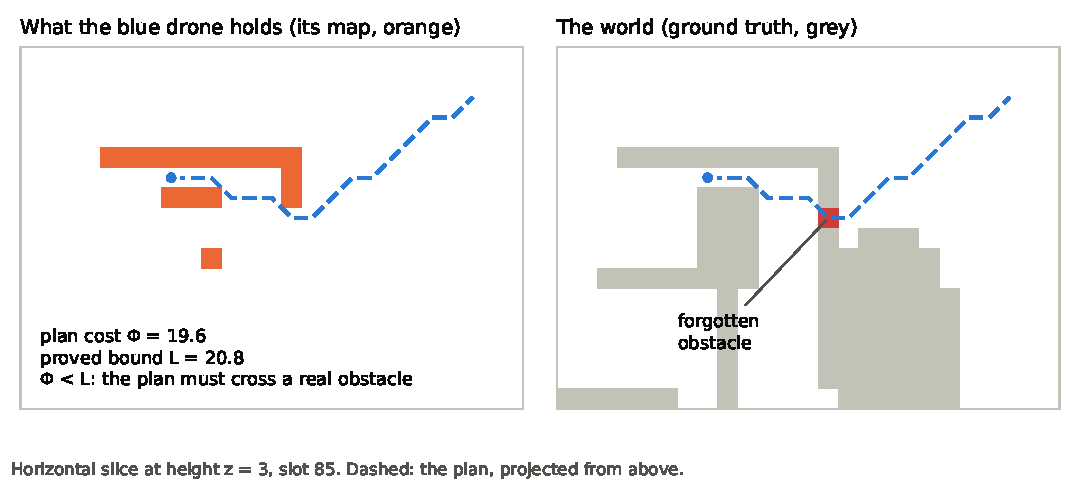
\includegraphics[width=\linewidth]{fig/futility.pdf}
\caption{Futility, as it happened (seed 2, the blue drone of Figure~\ref{fig:strip}, slot 85). Left: the drone's map at
the height where its plan meets the obstacle; the plan (dashed) is the cheapest route through it. Right: the ground
truth. The plan crosses one blocked voxel (red), which the drone held until the previous slot and evicted to make room.
The drone cannot see it, but $\Phi<L$ proves the plan blocked (F45.1), and with honest maps only an eviction can cause
it (F45.2). The same voxel later traps two teammates, and futility frees them the same way.}
\label{fig:futility}
\end{figure}

\begin{result}{Proposition F45.3}[liveness kept]
T2.9 holds with the futility trigger.
\end{result}
\begin{proof}
The rule only adds triggers, each
starting an escape with probability $1\ge p_{\rm esc}$; Lemma 9.3 needs infinitely many triggers on runs that do not
arrive, which extra triggers cannot remove, and the bound of the theorem's proof uses only $p_{\rm esc}$ as a lower
bound on the probability of starting an escape at a trigger.
\end{proof}
\trace{\code{agent.py} step 6}{\code{futile_crosses}, \code{inv_search}, \code{inv_move}, \code{inv_learn},
\code{no_futility}, \code{fail_bound}}{\code{test_futility_invariant}}{Section~\ref{sec:f45}}

\begin{result}{Proposition F45.6}[commit opportunities in a launch schedule]
Agents launch at $i\Delta$, $i=0..N-1$; a commit (T2.8) needs, at $A$ before launch, every chunk of a VERIFIED route;
chunks travel one hop from an arrived agent whose walk record holds. (a) The first arrival $T_1\ge\norm{B-A}_\infty$.
(b) If the chunks reach $A$ by slot $m=T_1+\delta$, $\delta\ge1$, agent $i$ can commit only if $i\Delta>m$: at most
$N-(\lfloor m/\Delta\rfloor+1)$ agents can, none if $m\ge(N-1)\Delta$. (c) None can if no packet from an arrived agent
reaches $A$ before $(N-1)\Delta$.
\end{result}
\begin{proof}
(a) Along any coordinate the position after $t$ moves differs from the start by at most
$t$ (induction on $t$, Lean \code{reach_time}), and reaching $B$ needs a difference of $\|B-A\|_\infty$ along some
coordinate. (b) The route exists only after an arrival; an agent that has launched has left $A$; the $i<N$ with
$i\Delta>m$ are those with $i>\lfloor m/\Delta\rfloor$ (Lean \code{commit_count}). (c) is the one-hop hypothesis.
\end{proof}
\trace{\code{agent.py} VERIFIED handling}{\code{reach_time}, \code{commit_count}}{\code{benchmarks/f45_commit_reach.py}}{Section~\ref{sec:f45}}

\section{How the embedded figures are counted}\label{sec:budget}

\paragraph{Bytes on the wire.} Packets are encoded bit-exactly and the encoded length is what the radio carries and
what is counted. Z3 proves that packing and unpacking of every header and claim word are inverse for all field values;
3000 random packets equal an independent encoder written from the specification table and every truncation is
rejected; shifting the pose by any multiple of 32 voxels leaves the bytes unchanged
(\code{test_wire_layout_z3}, \code{test_wire_bit_exact_and_roundtrip}, \code{test_zero_global_coordinate_bytes}).

\paragraph{Cycles.} Each primitive is counted inside the agent at a declared Cortex-M4 price: bit test 4, hash or heap
operation 30, segment--box slab test 40, segment step 8, relaxation 12, $h_3$ 20, byte handled 2 cycles
(\code{src/sim3d/ops.py}). The prices are an estimate to be calibrated against a C port of steps 1 and 4; Python wall
time is never used. An A* expansion costs at most $30+26(12+30+4+30+20)=2526$ cycles, and the search stops once 70\,\%
of the slot is spent; the remaining 30\,\% covered every compression measured, but it is not a worst-case guarantee.

\begin{figure}[htbp]\centering
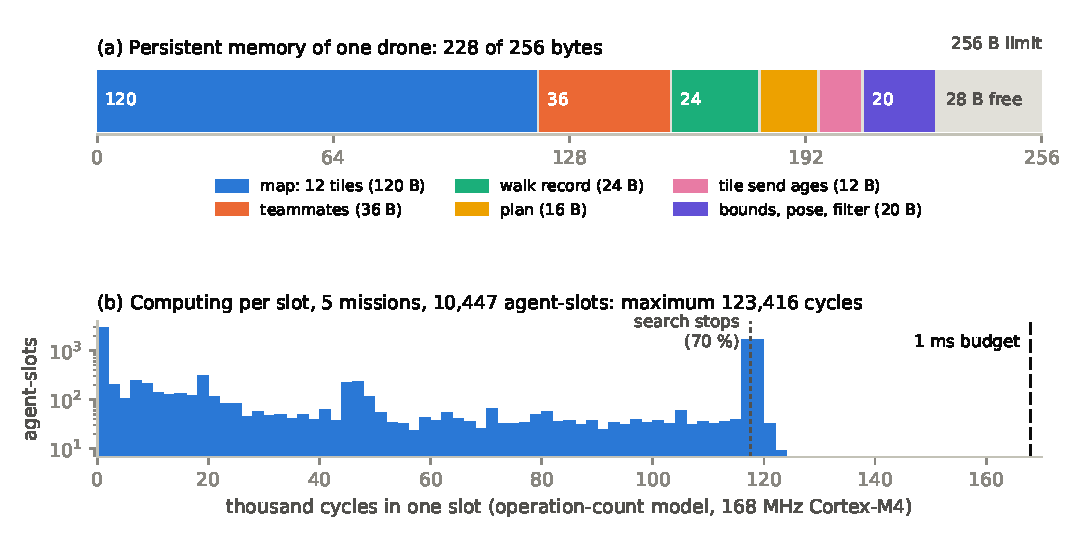
\includegraphics[width=\linewidth]{fig/budget.pdf}
\caption{The embedded budget. (a) The persistent state of one drone, structure by structure (Section~\ref{sec:protocol}),
against the 256\,B limit. (b) Cycles in each agent-slot of five missions (log scale): the planning search stops at 70\,\%
of the slot, and no slot comes near the 1\,ms budget.}
\label{fig:budget}
\end{figure}

\paragraph{Memory.} \code{Agent.memory_used} recomputes the layout of Section~\ref{sec:protocol} from the live state;
the checked mission asserts at most 256\,B at every slot. A* sets, the box-visibility graph and packet buffers live in
the arena; a search holds at most 2048 nodes and stops before an expansion that would overflow it (T2.6 still holds).

\section{Measurements}\label{sec:measure}

20 paired terrains (seeds 0--19): each configuration runs on the same terrains, links and sensors. Ten agents launch
10 slots apart; missions last 500 slots unless stated. Regret is the mean over agents of distance flown, plus the
true distance left if not arrived, over the true shortest distance, minus one. Baselines from v0.4 receive 120\,B of
map memory (their other state is not bounded); GRACE-3D 2.0.0 keeps 228\,B in total. ``v2 minus it'' is the paired
difference in regret.

\paragraph{How two configurations are compared.}
Let $R_X(s)$ be the regret of configuration $X$ on terrain $s$, the mean over its ten agents. Every configuration
flies the same $n=20$ terrains, so the comparison is made terrain by terrain:
\[
d_X(s)=R_{\rm v2}(s)-R_X(s),\qquad
\bar d_X=\frac1n\sum_{s=1}^{n}d_X(s),\qquad
\mathrm{se}_X=\frac{1}{\sqrt n}\biggl(\frac{1}{n-1}\sum_{s=1}^{n}\bigl(d_X(s)-\bar d_X\bigr)^2\biggr)^{1/2},
\]
and Figure~\ref{fig:forest} draws $\bar d_X\pm1.96\,\mathrm{se}_X$. A negative $\bar d_X$ means that GRACE-3D 2.0.0
detours less than $X$. Pairing removes what the two runs share, the terrain: the regret of GRACE-3D 2.0.0 alone ranges
from 0.20 to 2.21 across terrains (s.d.\ 0.64), CAIRN v0.4's spreads with s.d.\ 0.55, and yet their paired
differences spread with only 0.39. The same fact warns against reading Figure~\ref{fig:planes} by overlapping bars:
there each bar is the s.e.\ of one mean, $\mathrm{sd}(R_X)/\sqrt n$, which still contains the terrain spread, so two
points whose bars overlap may differ clearly once paired. Each interval covers one comparison. With the $t$ quantile
for 19 degrees of freedom (2.09 instead of 1.96) no interval changes side of zero; with Holm's correction for the nine
comparisons of Figure~\ref{fig:forest} at family level 0.05 (paired $t$-tests), four differences remain: oldest-first
forgetting, flooding, CAIRN v0.4 and the box-visibility planner.

\begin{figure}[htbp]\centering
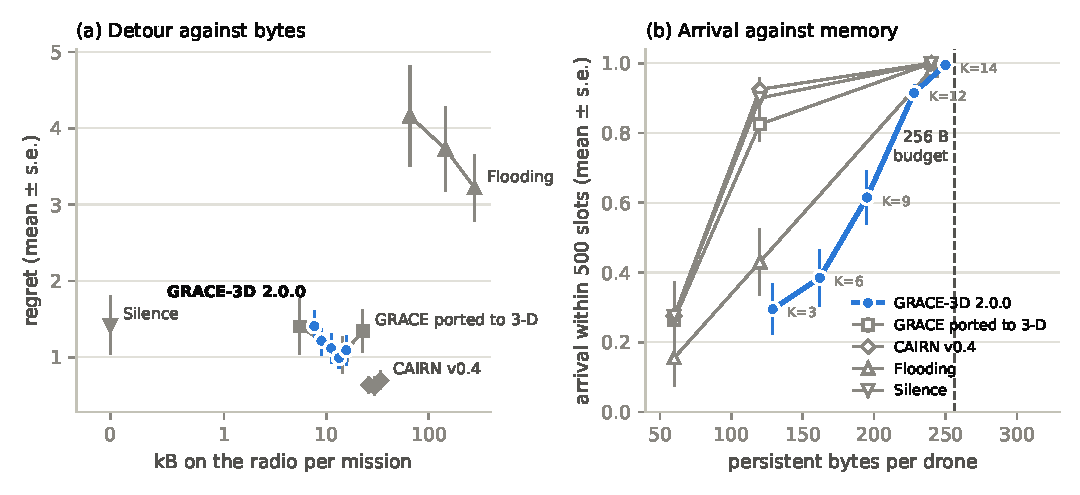
\includegraphics[width=\linewidth]{fig/planes.pdf}
\caption{The two main planes. Every point is a mean over the same 20 terrains, with $\pm1$ standard error over those
paired seeds on each axis that varies. (a) Detour against bytes, along the fronts traced by the price $\kappa$
(GRACE-3D 2.0.0: $\kappa=4,2,1,0.5,0.25$ from left to right; GRACE ported to 3-D and CAIRN v0.4: $\kappa=10,2,0.5$) and
by the packet budget (flooding: 16, 36, 66 B per slot); silence is one point. (b) Arrival within 500 slots against
persistent memory: GRACE-3D 2.0.0 for $K=3,6,9,12,14$ tiles, i.e.\ its whole state of $11K+96$ bytes; the v0.4 agents
for 60, 120 and 240\,B of map (hollow markers: their other state is not bounded). \code{benchmarks/sweep_v2.py}.}
\label{fig:planes}
\end{figure}

\begin{figure}[htbp]\centering
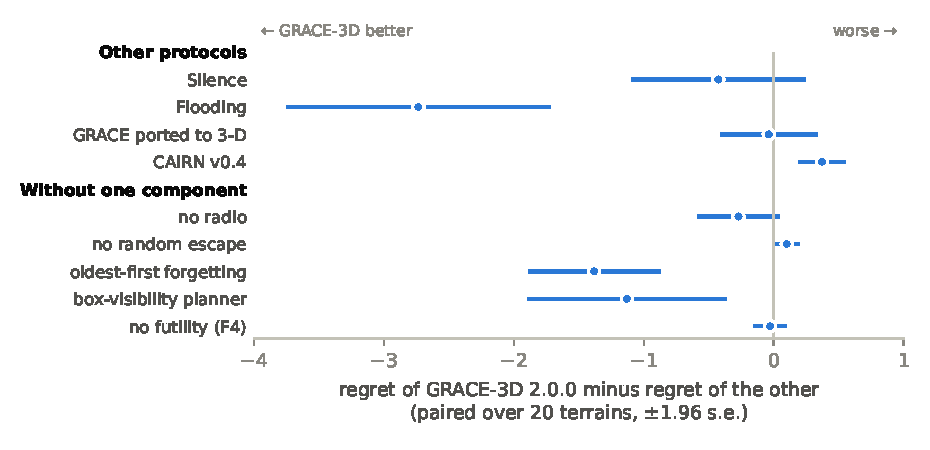
\includegraphics[width=.86\linewidth]{fig/results.pdf}
\caption{Paired differences in regret, GRACE-3D 2.0.0 minus each other protocol (top) and minus itself without one
component (bottom); bars are 95\,\% intervals ($\pm1.96$ s.e.) over the 20 terrains.}
\label{fig:forest}
\end{figure}

\begin{figure}[htbp]\centering
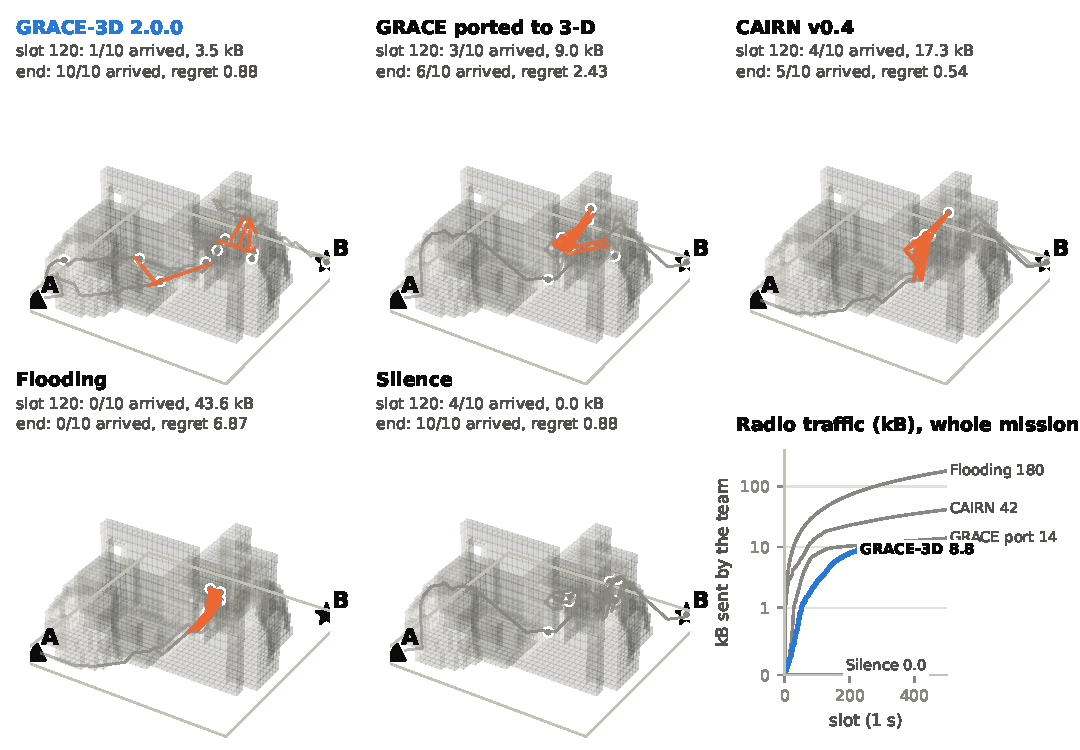
\includegraphics[width=\linewidth]{fig/compare.pdf}
\caption{One terrain (seed 2) flown by the five protocols, at slot 120: the drones with their last 30\,s of flight
and the radio deliveries of the last 5\,s (orange: obstacle maps; grey: position messages). Flooding saturates the
channel and no drone arrives; silence sends nothing; GRACE-3D 2.0.0 sends least among those that talk. Right: the
team's cumulative radio traffic. Single-terrain numbers vary: on this terrain silence also brings all ten drones home,
with the same regret as GRACE-3D 2.0.0 (0.88), while over the 20 terrains its regret is 1.42 against 0.99.
Figures~\ref{fig:planes} and \ref{fig:forest} give the paired statistics. Animated: \code{results/v2/grace3d_vs.gif}.}
\label{fig:compare}
\end{figure}

\paragraph{Reading Figure~\ref{fig:planes}.} (a) The price sweep of GRACE-3D 2.0.0 runs from 7.6\,kB per mission
($\kappa=4$) to 15.7\,kB ($\kappa=0.25$). Its regret is lowest at the default $\kappa=0.5$ ($0.99\pm0.14$ at 13.3\,kB):
spending more does not lower it ($1.09\pm0.20$ at 15.7\,kB), and spending less raises it to $1.41\pm0.21$ at
7.6\,kB. GRACE ported to 3-D lies in the
same band ($1.03\pm0.24$ at 14.3\,kB, 1.34 at 22.7\,kB, 1.40 at 5.5\,kB), so these 20 terrains do not separate the
two fronts. CAIRN v0.4 reaches 0.62--0.70 with 26--34\,kB, below every point of the GRACE-3D sweep: its advantage
cannot be bought with bytes, which agrees with its source being the relay of verified routes (F45.6). Flooding needs
66--281\,kB and stays above 3.2; silence costs 1.42 with no byte. (b) With $K=3,6,9,12,14$ tiles GRACE-3D 2.0.0 keeps
129 to 250\,B in total, and its arrival within 500 slots rises from 0.30 to 0.995. Below 9 tiles an agent cannot hold
the obstacles around it, and most agents are still flying at slot 500 (they arrive later, as T2.9 guarantees: 87\,\%
within 5000 slots at $K=6$). At the default 12 tiles arrival is 0.915; at 14 tiles, 250\,B, it is $0.995\pm0.005$ with
a regret of $0.73\pm0.10$. The baselines' points count only their map: with 120\,B of map they reach 0.83--0.93
(flooding 0.43), with 240\,B all of them arrive (flooding 0.98), and with 60\,B they all fall to 0.15--0.28. Their
remaining state is not bounded, so the horizontal positions are not comparable byte for byte, while GRACE-3D's
include everything. Within the 256-byte budget, two more tiles are worth more than the 28 bytes the default leaves
free; $K=12$ was fixed by the specification before this sweep, and changing it is left to the next version
(Section~\ref{sec:dev}).

\paragraph{Reading Figure~\ref{fig:forest}: other protocols.}
\emph{Flooding} detours 2.74 more than GRACE-3D 2.0.0 (95\,\% interval 1.73 to 3.74; worse on 17 of the 20
terrains) while sending 11 times the bytes, and only 43\,\% of its agents arrive within 500 slots. \emph{Silence}
(the v0.4 agent with 120\,B of map) detours 0.43 more on average, but the interval runs from $-1.08$ to $+0.23$ and
GRACE-3D 2.0.0 is better on only 10 of the 20 terrains. Talking does not help on every terrain; it removes the bad
ones: on its worst terrain silence reaches a regret of 6.73 against 2.21, and its 95th percentile is 4.56 against
2.15. \emph{GRACE ported to 3-D} has the same regret ($-0.04$, interval $-0.40$ to $+0.32$; GRACE-3D 2.0.0 is lower
on 6 of the 20 terrains), but GRACE-3D 2.0.0 brings 9 percentage points more of its agents home (0.915 against 0.825;
paired difference $0.090\pm0.040$ s.e.), sends 7\,\% fewer bytes and keeps its whole state in 228\,B, where the port
is given 120\,B of map and an unbounded rest. \emph{CAIRN v0.4} detours 0.37 less than GRACE-3D 2.0.0 (interval 0.20
to 0.54; lower on 18 of the 20 terrains) and arrives as often (0.925 against 0.915), at 2.2 times the bytes and with
its state beyond the map unbounded. Its advantage is that it relays verified routes in flight, which v2 does not do
(Proposition F45.6 and Section~\ref{sec:dev}).

\paragraph{Reading Figure~\ref{fig:forest}: components.}
\emph{Goal-relevant forgetting} is the largest single effect: oldest-first eviction instead adds 1.38 of regret
(interval 0.89 to 1.88), on every one of the 20 terrains, and arrival falls from 0.915 to 0.615. With 12 tiles,
which tiles stay matters more than anything else measured here. \emph{The exact sliced A*} saves 1.13 against the
box-visibility planner (interval 0.38 to 1.88; 17 of the 20 terrains), which is also the only planner that overruns
the slot (below). \emph{The radio}, against the same agent without it, removes 0.27 of regret on average and helps on
13 of the 20 terrains, but its interval ($-0.58$ to $+0.03$) includes zero: 20 terrains do not separate this effect
from chance. \emph{The random escape trigger} costs 0.10 (interval 0.01 to 0.19; $p=0.042$, not significant after
Holm's correction). It is kept because T2.9 rests on it: without it, an agent whose plan neither shortens nor meets
anything new never escapes, and on 40 small random worlds a reduced agent cycles for ever in 15 of them without
escapes, while it arrives in all 40 with them (after T2.9). In this bench the agents without it arrive as often (0.910 against 0.915),
so the bench measures the price of the guarantee, not its benefit. \emph{Futility} changes the regret by $-0.03$
(interval $-0.14$ to $+0.08$) at $K=12$ and 500 slots: it was adopted for its byte saving (Section~\ref{sec:f45}),
and it acts where memory is tight: with $K=6$, 87\,\% of the agents arrive within 5000 slots against 65\,\% without it.

\begin{table}[htbp]\centering\small
\begin{tabularx}{\linewidth}{Lrrrrrr}
\toprule
Configuration & regret & p95 & p99 & arrival & kB & v2 minus it \\
\midrule
\textbf{GRACE-3D 2.0.0} & $0.991\pm0.144$ & 2.15 & 2.19 & 0.915 & 13.3 & --- \\
v2 without radio & $1.263\pm0.204$ & 2.98 & 3.00 & 0.880 & 0.0 & $-0.272\pm0.155$ \\
v2 without the random escape trigger & $0.892\pm0.137$ & 1.93 & 2.21 & 0.910 & 12.7 & $+0.099\pm0.045$ \\
v2 with oldest-first forgetting & $2.374\pm0.324$ & 4.70 & 5.08 & 0.615 & 15.6 & $-1.383\pm0.253$ \\
v2 with the box-visibility planner & $2.122\pm0.499$ & 6.12 & 6.77 & 0.855 & 13.2 & $-1.131\pm0.383$ \\
v2 without futility (the F4 agent) & $1.020\pm0.162$ & 2.37 & 2.48 & 0.885 & 13.9 & $-0.029\pm0.057$ \\
GRACE ported to 3-D, 120 B of map & $1.030\pm0.242$ & 3.18 & 3.83 & 0.825 & 14.3 & $-0.039\pm0.184$ \\
CAIRN v0.4, 120 B of map & $0.620\pm0.123$ & 1.87 & 2.29 & 0.925 & 29.5 & $+0.371\pm0.087$ \\
flooding, 120 B of map & $3.726\pm0.556$ & 6.97 & 7.65 & 0.430 & 146.1 & $-2.735\pm0.511$ \\
silence (v0.4 agent), 120 B of map & $1.418\pm0.386$ & 4.56 & 6.30 & 0.900 & 0.0 & $-0.427\pm0.335$ \\
silence, unbounded map & $0.781\pm0.082$ & 1.33 & 1.43 & 1.000 & 0.0 & --- \\
v2 with $K=6$ tiles (60 B of map) & $2.985\pm0.352$ & 5.34 & 5.71 & 0.385 & 13.7 & --- \\
\bottomrule
\end{tabularx}
\caption{The bench: 20 paired terrains, ten agents, 500 slots; the columns are defined in the text of
Section~\ref{sec:measure}.}
\label{tab:bench}
\end{table}

\paragraph{Reading Tables~\ref{tab:bench} and~\ref{tab:constraints}.} In Table~\ref{tab:bench},
\emph{regret} is the mean of $R_X(s)$ over the 20 terrains $\pm$ its s.e., $\mathrm{sd}(R_X)/\sqrt{20}$; \emph{p95}
and \emph{p99} are percentiles of the 20 per-terrain regrets, interpolated linearly: with 20 values, p95 is
essentially the second-worst terrain and p99 lies close to the worst; \emph{arrival} is the share of the 200 agents (10 per terrain) at B within 500 slots;
\emph{kB} counts every byte the team put on the radio during one mission, headers included; \emph{v2 minus it} is
$\bar d_X\pm\mathrm{se}_X$. Silence with an unbounded map shows what perfect memory achieves without any radio (0.78,
every agent home); v2 with $K=6$ shows the cost of halving the map: 38.5\,\% arrive within 500 slots. In
Table~\ref{tab:constraints}, C1 first divides the tile bytes sent (10 per tile) by the obstacle voxels those tiles carry, the set bits of
their masks: 0.641\,B, i.e.\ 15.6 obstacle voxels per tile. C1 then compares the information efficiency
$\eta_{3D}=(\bar R_{\text{v2 without radio}}-\bar R_{\rm v2})/\mathrm{kB}_{\rm v2}=0.0204$ regret removed per kB with
v1's 0.013--0.026 per kB (midpoint 0.0195). Its numerator is the radio effect above, whose interval includes zero, so
within $\pm1$ s.e.\ the ratio $1.05$ is only known to lie between 0.45 and 1.65. C2 takes, in each mission, the 99th
percentile over slots of the cycles spent in step 1 (ingesting the sensor scan), and reports the 99th percentile of
those over the 20 missions. C3 is the worst slot over the 20 missions of GRACE-3D 2.0.0, its persistent state and its
arrival; C4 checks that shifting every position by a multiple of 32 voxels leaves every byte on the wire unchanged (T2.3, T2.4). The
verified-route fit rate is the share of arrived agents whose flown path fits the 12-waypoint record: 9.3\,\%, and
Proposition F45.6 explains why such routes are never used in this schedule. Both tables are written by
\code{benchmarks/eval_v2.py} to \code{benchmarks/v2_results.json}.

\begin{table}[htbp]\centering\small
\begin{tabularx}{\linewidth}{Lrrl}
\toprule
Constraint & Value & Target & Met \\
\midrule
C1 tile bytes per obstacle voxel carried & 0.641 & $\le$ 0.7 & yes \\
C1 $\eta_{3D}/\eta_{2D}$ (regret removed per kB, against v2's own silence) & 1.048 & $\ge$ 0.5 & yes \\
C2 step-1 cycles per slot, p99 & 1\,456 & $<$ 20\,000 & yes \\
C3 cycles per slot, maximum & 124\,152 & $<$ 168\,000 & yes \\
C3 persistent state, bytes & 228 & $\le$ 256 & yes \\
C3 liveness: arrival within 20\,000 slots, $K=12$ & 1.0 & 1.0 & yes \\
C3 stress: arrival within 5000 slots, $K=6$ & 0.87 & report & --- \\
C3 arrival within 500 slots, $K=12$ & 0.915 & report & --- \\
C3 arrival within 500 slots, $K=6$ & 0.385 & report & --- \\
C3 verified-route fit rate & 0.093 & report & --- \\
C4 global-coordinate bytes on the wire & 0 & 0 & yes \\
\bottomrule
\end{tabularx}
\caption{The constraints of the v2 specification and their measured values.}
\label{tab:constraints}
\end{table}

Every configuration of GRACE-3D 2.0.0 in the bench (with and without radio, without the random trigger, with
oldest-first forgetting, with $K=6$, and the 20\,000- and 5000-slot runs) stays within 124\,954 cycles per slot over
694\,326 agent-slots, with no overrun, and within 228\,B. Only the ablation that runs the box-visibility planner alone,
in one slot, overruns (1\,588 of 40\,264 agent-slots, up to 396\,460 cycles), which is why v2 slices an exact search
over slots instead. All 200 agents arrive within 20\,000 slots at $K=12$; with 6 tiles, 87\,\% arrive within 5000
slots, against 65\,\% for the F4 agent: the regime of heavy forgetting is where futility acts (F45.2).

\section{F4.5: one post-empirical pass}\label{sec:f45}

The F4 agent was audited constant by constant (\code{docs/v2_proofs.md}, F4.5.0). Two mechanisms it left unused
became candidates, each proved, mechanised and checked before it ran: the futility trigger (F45.1--F45.3) and the v1
loss model in tile selection, which rests on Propositions F45.4 and F45.5 below. In that model a pool tile $a$ carries
one byte $u(a)\in[0,1]$, the believed probability that a teammate still lacks it ($u\gets1$ when the tile changes);
its gain is $g(a)=u(a)\sum_jV_j(a)(1-\beta_j)$, where $\beta_j$ is the probability that a copy sent now is lost on
the link to teammate $j$, and after a copy $u\gets u\,\bar\beta$ with $\bar\beta=\sum_jV_j\beta_j/\sum_jV_j$.

\noindent\emph{How it is found.} A link that was just heard was good at that moment; what matters is how fast that
knowledge decays. Writing the probability of the bad state as a first-order recurrence and solving it gives a closed
form. Second, 256 bytes cannot hold one belief per tile and teammate, so the per-receiver beliefs must collapse into
one number per tile; the question is which collapse loses nothing that the selection rule uses.

\begin{result}{Proposition F45.4}[loss after hearing]
Let the directed link be a two-state Markov chain~\cite{gilbert,elliott} with $P(G\to B)=p$, $P(B\to G)=q$, $p+q>0$,
and let the receiver have been heard at $t_j$, so that the link was good then. Then
$P(B_{t_j+\tau}\mid G_{t_j})=\pi_B(1-\lambda^\tau)$, with $\pi_B=p/(p+q)$ and $\lambda=1-p-q$.
\end{result}
\begin{proof}
Let $x_\tau=P(B_{t_j+\tau}\mid G_{t_j})$. Then $x_0=0$ and, conditioning on the state at $\tau$,
$x_{\tau+1}=x_\tau(1-q)+(1-x_\tau)p=p+\lambda x_\tau$. The sequence $y_\tau=\pi_B(1-\lambda^\tau)$ has $y_0=0$ and
$p+\lambda y_\tau=p+\lambda\pi_B-\pi_B\lambda^{\tau+1}=\pi_B(p+q)+\pi_B(1-p-q)-\pi_B\lambda^{\tau+1}
=\pi_B(1-\lambda^{\tau+1})=y_{\tau+1}$, using $p=\pi_B(p+q)$. Both sequences satisfy the same first-order recurrence
with the same start, so they are equal (induction on $\tau$).
\end{proof}
\trace{\code{f45_v2.py} candidate}{\code{badAfter_eq}}{\code{test_ge_closed_form} (SymPy and Monte Carlo)}{Section~\ref{sec:f45}}

\begin{result}{Proposition F45.5}[scalar belief]
Suppose that before a copy every receiver lacks the tile with probability $u$, and that a copy reaches $j$ with
probability $1-\beta_j$, independently of whether $j$ lacked it. (a) The copy's expected delivered value is
$u\sum_jV_j(1-\beta_j)$. (b) After it, $j$ lacks the tile with probability $u\beta_j$, and the scalar update
$u'=u\bar\beta$ keeps the expected value still to deliver exactly: $\sum_jV_ju\beta_j=(\sum_jV_j)\,u'$.
\end{result}
\begin{proof}
(a) Teammate $j$ gains $V_j$ if and only if it lacked the tile and the copy arrived, which has probability
$u(1-\beta_j)$; sum over $j$. (b) $j$ still lacks the tile if and only if it lacked it and the copy was lost:
$u\beta_j$. Then $(\sum_jV_j)\,u\bar\beta=(\sum_jV_j)\,u\,\frac{\sum_jV_j\beta_j}{\sum_jV_j}=\sum_jV_ju\beta_j$.
\end{proof}
\noindent The collapse is exact for the expected remaining value at the current weights; it approximates the
per-receiver beliefs, which 256\,B cannot hold ($K\times(N-1)$ bytes). With all tiles of 10\,B, maximising expected
delivered value minus $\kappa$ per byte selects the tiles of largest $g(a)\ge10\kappa$ up to the room left: v1's
Theorem~1~\cite{v1}, whose proof (a linear, separable objective under a cardinality constraint) applies verbatim
with the new $g$.
\trace{\code{f45_v2.py} candidate}{\code{belief_update}}{\code{test_belief_update_identity} (SymPy)}{Section~\ref{sec:f45}}

\noindent
Rule fixed before the runs: 40 paired terrains (20 main, 20 unseen); adopt a candidate only if it improves a Pareto
metric (regret, bytes, p99 slot cycles) with paired $t$-test $p<0.05/3$ and the same sign on both halves, degrades
none and keeps every constraint; compose candidates only if the composite also passes and is not worse than either
component alone.

\begin{table}[htbp]\centering\small
\begin{tabularx}{\linewidth}{>{\raggedright\arraybackslash}p{3.3cm}LLl}
\toprule
Against F4 & regret & bytes per mission & outcome \\
\midrule
futility & $-0.072\pm0.044$ ($p=0.11$) & $-1011\pm362$ ($p=0.008$) & \textbf{adopted} \\
loss model & $+0.081\pm0.048$ ($p=0.10$) & $-2422\pm681$ ($p=0.001$) & passes alone \\
futility, $p_{\rm esc}=0.01$ & $-0.125\pm0.060$ ($p=0.044$) & $-1156\pm435$ ($p=0.011$) & passes; tie \\
loss and futility & $+0.115\pm0.065$ ($p=0.087$) & $-2428\pm742$ ($p=0.002$) & rejected \\
\bottomrule
\end{tabularx}
\caption{The F4.5 candidates against the F4 agent, paired over 40 terrains: mean $\pm$ s.e.\ and paired $t$-test.}
\label{tab:f45}
\end{table}

The composite is significantly worse in regret than futility alone ($+0.186\pm0.060$, $p=0.004$), so the rule adopts
futility alone. The two futility variants differ significantly only in the number of escapes, so the one that changes
no constant ($p_{\rm esc}=0.05$) is kept. The link counters that only the loss model would read were deleted
($255\to228$\,B). On the final code, the F4 agent (\code{v2-nofutile}) and both futility variants reproduce all 120
evaluation missions exactly, memory aside. Futility saves bytes mostly by shortening travel: agent-slots before arrival
drop from 2339 to 2229 per mission ($p=0.015$), which at the F4 rate accounts for 69\,\% of the saving, because a tile
is worth nothing to an arrived teammate. A likely reason the loss model fails, not tested: it assumes receivers keep a
tile once they have it, whereas receivers with 12 tiles evict, and the fixed 8-slot resend re-supplies what they
evicted.

Commits never occur (F45.6). $T_1\ge60$ slots in all 40 missions, so only agents 7--9 could ever commit; in the five
missions with $T_1\le88$, arrived agents sent 63 to 734 VERIFIED claims, yet no packet from an arrived agent reached an
agent still at $A$: $B$ lies about 250\,m from $A$ across the terrain, and routes travel one hop.

\section{Limitations and next steps}\label{sec:dev}

\begin{itemize}
\item \textbf{Local repair (a deviation from target 3):} incremental search in the sense of Ramalingam and
Reps~\cite{rr96} (and D*~Lite~\cite{dstarlite}) stores a distance map, $\Theta(\abs\Omega)$ state, which does not fit in
256\,B. v2 re-plans exactly from scratch in the arena instead; a search expands 208 nodes at the median and 940 at
p99, and fits the arena in 99.6\,\% of searches.
\item \textbf{Completeness:} it is probabilistic (T2.9), or deterministic along a verified route (T2.8); deterministic
completeness with finite state is impossible for one agent (T2.10). T2.9 bounds liveness, not speed: at $K=6$,
87\,\% of the agents arrive within 5000 slots.
\item \textbf{Verified routes:} they are idle in this schedule (F45.6). Relaying them, or adopting routes in flight, is
what CAIRN v0.4 does and what its lower regret reflects; it is the next step (v3).
\item \textbf{Tile budget:} the sweep of Figure~\ref{fig:planes}(b) shows that $K=14$ tiles (250\,B) brings 99.5\,\% of
the agents home within 500 slots against 91.5\,\% at the specified $K=12$; adopting it needs the same pre-registered
paired test as F4.5.
\item \textbf{Cycles:} they come from a model, not from a microcontroller: no C port exists yet, and the absence of
dynamic allocation in the slot loop is a property of the fixed layout and arena, not of the Python simulator.
\item \textbf{Model:} generated terrain, simulated radio, exact sensing and odometry, static obstacles and honest
teammates.
\end{itemize}

\section{Reproducibility}

\begin{verbatim}
pip install -e ".[test]"
pytest -q                             # unit tests and math checks
cd formal && lake exe cache get && lake build && cd ..
python benchmarks/eval_v2.py          # the bench: v2_results.json
python benchmarks/sweep_v2.py         # the two planes: v2_sweep.json
python benchmarks/f45_v2.py           # F4.5 decision: v2_f45.json
python benchmarks/f45_commit_reach.py # F45.6 (c): v2_f45_commit.json
python experiments/v2_media.py        # figures, GIFs, 3-D replay
\end{verbatim}
Every mission is seeded, so every number, figure and frame is reproduced exactly. Specification:
\code{docs/v2_spec.md}; longer proofs and the F4.5 audit: \code{docs/v2_proofs.md}.

\paragraph{Responsible use.} This is open, basic research on information-efficient coordination of autonomous systems
over degraded networks, for dual-use applications such as search and rescue, emergency response and infrastructure
inspection. It uses only synthetic data and contains no weapon, targeting or vehicle-specific control code.

\begin{thebibliography}{99}\small
\bibitem{v1} Ropera Labs. GRACE: Goal-Relevant Adaptive Compressed Exchange. Technical report RL-TR-2026-03,
swarm-dil v0.3, 2026.
\bibitem{budach} L.~Budach. Automata and labyrinths. \emph{Mathematische Nachrichten}, 86:195--282, 1978.
\bibitem{hoffmann} F.~Hoffmann. One pebble does not suffice to search plane labyrinths. \emph{FCT}, LNCS 117,
433--444, 1981.
\bibitem{fipp} P.~Fraigniaud, D.~Ilcinkas, G.~Peer, A.~Pelc and D.~Peleg. Graph exploration by a finite automaton.
\emph{Theoretical Computer Science}, 345(2--3):331--344, 2005.
\bibitem{blumkozen} M.~Blum and D.~Kozen. On the power of the compass (or, why mazes are easier to search than
graphs). \emph{FOCS}, 1978.
\bibitem{reingold} O.~Reingold. Undirected connectivity in log-space. \emph{Journal of the ACM}, 55(4):17:1--17:24,
2008.
\bibitem{aleliunas} R.~Aleliunas, R.~M.~Karp, R.~J.~Lipton, L.~Lov\'asz and C.~Rackoff. Random walks, universal
traversal sequences, and the complexity of maze problems. \emph{FOCS}, 1979.
\bibitem{kamon} I.~Kamon, E.~Rimon and E.~Rivlin. Range-sensor-based navigation in three-dimensional polyhedral
environments. \emph{The International Journal of Robotics Research}, 20(1):6--25, 2001.
\bibitem{rr96} G.~Ramalingam and T.~Reps. An incremental algorithm for a generalization of the shortest-path problem.
\emph{Journal of Algorithms}, 21(2):267--305, 1996.
\bibitem{dstarlite} S.~Koenig and M.~Likhachev. D* Lite. \emph{AAAI}, 2002.
\bibitem{hart} P.~E.~Hart, N.~J.~Nilsson and B.~Raphael. A formal basis for the heuristic determination of minimum
cost paths. \emph{IEEE Transactions on Systems Science and Cybernetics}, 4(2):100--107, 1968.
\bibitem{shapiro} M.~Shapiro, N.~Pregui\c{c}a, C.~Baquero and M.~Zawirski. Conflict-free replicated data types.
\emph{SSS}, 2011.
\bibitem{muller} H.~M\"uller, V.~Niculescu, T.~Polonelli, M.~Magno and L.~Benini. Robust and efficient depth-based
obstacle avoidance for autonomous miniaturized UAVs. arXiv:2208.12624, 2022.
\bibitem{gilbert} E.~N.~Gilbert. Capacity of a burst-noise channel. \emph{Bell System Technical Journal},
39(5):1253--1265, 1960.
\bibitem{elliott} E.~O.~Elliott. Estimates of error rates for codes on burst-noise channels. \emph{Bell System
Technical Journal}, 42(5):1977--1997, 1963.
\end{thebibliography}

\end{document}
